\chapter{微分中值定理及其应用}

\section{拉格朗日定理和函数的单调性}

在这一章里,我们要讨论怎样由导数 \({f}^{\prime }\) 的已知性质来推断函数 \(f\) 所应具有的性质. 微分中值定理 (包括罗尔定理、拉格朗日定理、柯西定理、泰勒定理) 正是进行这一讨论的有效工具.

本节首先介绍拉格朗日定理以及它的预备定理一罗尔定理, 并用此讨论函数的单调性.

\subsection{罗尔定理与拉格朗日定理}

%定理 6.1
\begin{theorem}{罗尔 (Rolle) 中值定理}{the:罗尔中值定理}
若函数 \(f\) 满足如下条件:

(i) \(f\) 在闭区间 \(\left\lbrack  {a,b}\right\rbrack\) 上连续;

(ii) \(f\) 在开区间(a, b)上可导;

(iii) \(f\left( a\right)  = f\left( b\right)\) ,

则在(a, b)上至少存在一点 \(\xi\) ,使得
\[
{f}^{\prime }\left( \xi \right)  = 0. \tag{1}
\]
\end{theorem}

罗尔定理的几何意义是说: 在每一点都可导的一段连续曲线上, 如果曲线的两端点高度相等,则至少存在一条水平切线 (图 6-1).

\begin{figure}
    \centering
    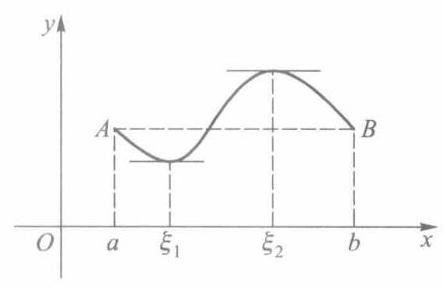
\includegraphics[width=.3\textwidth]{images/P032.jpg}
    \caption{图 $6-1$}
    \label{fig:P032}
\end{figure}

%证
\begin{proof}
因为 \(f\) 在 \(\left\lbrack  {a,b}\right\rbrack\) 上连续,所以有最大值与最小值,分别用 \(M\) 与 \(m\) 表示,现分两种情况来讨论:

(1) 若 \(m = M\) ,则 \(f\) 在 \(\left\lbrack  {a,b}\right\rbrack\) 上必为常数,从而结论显然成立.

(2)若 \(m < M\) ,则因 \(f\left( a\right)  = f\left( b\right)\) ,使得最大值 \(M\) 与最小值 \(m\) 至少有一个在(a, b)上的某点 \(\xi\) 处取得,从而 \(\xi\) 是 \(f\) 的极值点. 由条件 (ii), \(f\) 在点 \(\xi\) 处可导, 故由费马定理推知
\[
{f}^{\prime }\left( \xi \right)  = 0.
\]
\end{proof}

%注
\begin{remark}
定理中的三个条件缺少任何一个, 结论将不一定成立 (见图 6-2).
\end{remark}

\begin{figure}
    \centering
    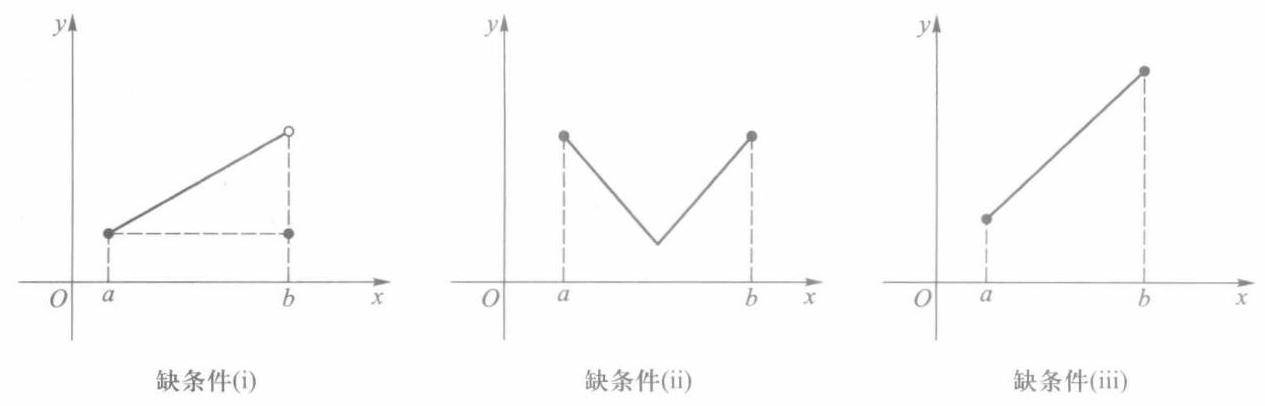
\includegraphics[width=.8\textwidth]{images/P033.jpg}
    \caption{图 $6-2$}
    \label{fig:P033}
\end{figure}

作为罗尔定理的简单应用, 请看下面的例子.

%例 1
\begin{example}
设 \(f\) 为 \(\mathbf{R}\) 上的可导函数,证明: 若方程 \({f}^{\prime }\left( x\right)  = 0\) 没有实根,则方程 \(f\left( x\right)  = 0\) 至多只有一个实根.
\end{example}


%证
\begin{proof}
这可反证如下: 倘若 \(f\left( x\right)  = 0\) 有两个实根 \({x}_{1}\) 和 \({x}_{2}\) (设 \({x}_{1} < {x}_{2}\) ),则函数 \(f\) 在 \(\left\lbrack  {{x}_{1},{x}_{2}}\right\rbrack\) 上满足罗尔定理的三个条件,从而存在 \(\xi  \in  \left( {{x}_{1},{x}_{2}}\right)\) ,使 \({f}^{\prime }\left( \xi \right)  = 0\) ,这与 \({f}^{\prime }\left( x\right)  \neq  0\) 的假设相矛盾,命题得证.
\end{proof}


%定理 6.2
\begin{theorem}{拉格朗日 (Lagrange) 中值定理}{the:拉格朗日中值定理}
若函数 \(f\) 满足如下条件:

(i) \(f\) 在闭区间 \(\left\lbrack  {a,b}\right\rbrack\) 上连续;

(ii) \(f\) 在开区间(a, b)上可导,

则在(a, b)上至少存在一点 \(\xi\) ,使得
\[
{f}^{\prime }\left( \xi \right)  = \frac{f\left( b\right)  - f\left( a\right) }{b - a}. \tag{2}
\]
\end{theorem}

显然,特别当 \(f\left( a\right)  = f\left( b\right)\) 时,本定理的结论 (2) 即为罗尔定理的结论 (1). 这表明罗尔定理是拉格朗日定理的一个特殊情形.

%证
\begin{proof}
作辅助函数
\[
F\left( x\right)  = f\left( x\right)  - f\left( a\right)  - \frac{f\left( b\right)  - f\left( a\right) }{b - a}\left( {x - a}\right) .
\]
显然, \(F\left( a\right)  = F\left( b\right) \left( { = 0}\right)\) ,且 \(F\) 在 \(\left\lbrack  {a,b}\right\rbrack\) 上满足罗尔定理的另两个条件. 故存在 \(\xi  \in\) (a, b),使
\[
{F}^{\prime }\left( \xi \right)  = {f}^{\prime }\left( \xi \right)  - \frac{f\left( b\right)  - f\left( a\right) }{b - a} = 0,
\]
移项后即得到所要证明的 (2) 式.
\end{proof}


拉格朗日中值定理的几何意义是: 在满足定理条件的曲线 \(y = f\left( x\right)\) 上至少存在一点 \(P\left( {\xi ,f\left( \xi \right) }\right)\) ,该曲线在该点处的切线平行于曲线两端点的连线 \({AB}\) . 我们在证明中引入的辅助函数 \(F\left( x\right)\) ,正是曲线 \(y = f\left( x\right)\) 与直线 \({AB}\left( {y = f\left( a\right)  + \frac{f\left( b\right)  - f\left( a\right) }{b - a}\left( {x - a}\right) }\right)\) 之差 (如图 6-3 所示).

\begin{figure}
    \centering
    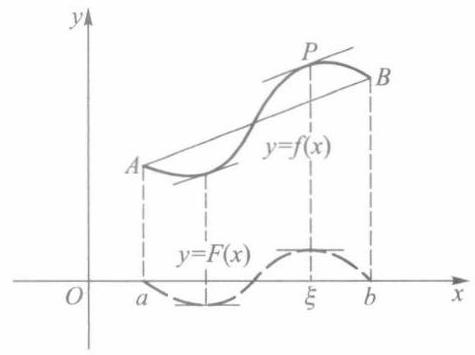
\includegraphics[width=.3\textwidth]{images/P034.jpg}
    \caption{图 $6-3$}
    \label{fig:P034}
\end{figure}

定理 6.2 的结论(公式(2))称为拉格朗日公式.

拉格朗日公式还有下面几种等价表示形式, 供读者在不同场合选用:
\[
f\left( b\right)  - f\left( a\right)  = {f}^{\prime }\left( \xi \right) \left( {b - a}\right) ,a < \xi  < b; \tag{3}
\]
\[
f\left( b\right)  - f\left( a\right)  = {f}^{\prime }\left( {a + \theta \left( {b - a}\right) }\right) \left( {b - a}\right) ,0 < \theta  < 1; \tag{4}
\]
\[
f\left( {a + h}\right)  - f\left( a\right)  = {f}^{\prime }\left( {a + {\theta h}}\right) h,0 < \theta  < 1. \tag{5}
\]
值得注意的是,拉格朗日公式无论对于 \(a < b\) , 还是 \(a > b\) 都成立,而 \(\xi\) 则是介于 \(a\) 与 \(b\) 之间的某一定数. 而 (4)、(5) 两式的特点,在于把中值点 \(\xi\) 表示成了 \(a + \theta \left( {b - a}\right)\) ,使得不论 \(a,b\) 为何值, \(\theta\) 总可为小于 1 的某一正数.


%例 2
\begin{example}
证明: \(\arctan b - \arctan a \leq  b - a\) ,其中 \(a\)  \(< b\) .
\end{example}


%证
\begin{proof}
设 \(f\left( x\right)  = \arctan x\) ,则
\[
f\left( b\right)  - f\left( a\right)  = {f}^{\prime }\left( \xi \right) \left( {b - a}\right)  = \frac{1}{1 + {\xi }^{2}}\left( {b - a}\right) ,\;a < \xi  < b.
\]
从而得
\[
\arctan b - \arctan a \leq  b - a.
\]
\end{proof}

%推论 1
\begin{corollary}{常量函数}{pro:常量函数}
1 若函数 \(f\) 在区间 \(I\) 上可导,且 \({f}^{\prime }\left( x\right)  \equiv  0,x \in  I\) ,则 \(f\) 为 \(I\) 上的一个常量函数.
\end{corollary}


%证
\begin{proof}
任取两点 \({x}_{1},{x}_{2} \in  I\left( \right.\) 设 \(\left. {{x}_{1} < {x}_{2}}\right)\) ,在区间 \(\left\lbrack  {{x}_{1},{x}_{2}}\right\rbrack\) 上应用拉格朗日定理,存在 \(\xi  \in\)  \(\left( {{x}_{1},{x}_{2}}\right)  \subset  I\) ,使得
\[
f\left( {x}_{2}\right)  - f\left( {x}_{1}\right)  = {f}^{\prime }\left( \xi \right) \left( {{x}_{2} - {x}_{1}}\right)  = 0.
\]
这就证得 \(f\) 在区间 \(I\) 上任何两点之值相等.
\end{proof}


由推论 1 又可进一步得到如下结论:

%推论 2
\begin{corollary}{可导关系}{pro:可导关系}
2 若函数 \(f\) 和 \(g\) 均在区间 \(I\) 上可导,且 \({f}^{\prime }\left( x\right)  \equiv  {g}^{\prime }\left( x\right) ,x \in  I\) ,则在区间 \(I\) 上 \(f\left( x\right)\) 与 \(g\left( x\right)\) 只相差某一常数,即
\[
f\left( x\right)  = g\left( x\right)  + c\;\left( {c\text{ 为某一常数 }}\right) .
\]
\end{corollary}


%推论
\begin{corollary}{导数极限定理}{pro:导数极限定理}
3 设函数 \(f\) 在点 \({x}_{0}\) 的某邻域 \(U\left( {x}_{0}\right)\) 上连续,在 \({U}^{ \circ  }\left( {x}_{0}\right)\) 上可导,且极限 \(\mathop{\lim }\limits_{{x \rightarrow  {x}_{0}}}{f}^{\prime }\left( x\right)\) 存在,则 \(f\) 在点 \({x}_{0}\) 可导,且
\[
{f}^{\prime }\left( {x}_{0}\right)  = \mathop{\lim }\limits_{{x \rightarrow  {x}_{0}}}{f}^{\prime }\left( x\right) . \tag{6}
\]
\end{corollary}

%证
\begin{proof}
分别按左、右导数来证明 (6) 式成立.

(1) 任取 \(x \in  {U}_{ + }^{0}\left( {x}_{0}\right) ,f\left( x\right)\) 在 \(\left\lbrack  {{x}_{0},x}\right\rbrack\) 上满足拉格朗日定理条件,则存在 \(\xi  \in  \left( {{x}_{0},x}\right)\) ,使得
\[
\frac{f\left( x\right)  - f\left( {x}_{0}\right) }{x - {x}_{0}} = {f}^{\prime }\left( \xi \right) . \tag{7}
\]
由于 \({x}_{0} < \xi  < x\) ,因此当 \(x \rightarrow  {x}_{0}^{ + }\) 时,随之有 \(\xi  \rightarrow  {x}_{0}^{ + }\) ,对 (7) 式两边取极限,便得
\[
\mathop{\lim }\limits_{{x \rightarrow  {x}_{0}^{ + }}}\frac{f\left( x\right)  - f\left( {x}_{0}\right) }{x - {x}_{0}} = \mathop{\lim }\limits_{{x \rightarrow  {x}_{0}^{ + }}}{f}^{\prime }\left( \xi \right)  = {f}^{\prime }\left( {{x}_{0} + 0}\right) .
\]
(2) 同理可得 \({f}^{\prime }\left( {x}_{0}\right)  = {f}^{\prime }\left( {{x}_{0} - 0}\right)\) .

因为 \(\mathop{\lim }\limits_{{x \rightarrow  {x}_{0}}}{f}^{\prime }\left( x\right)  = k\) 存在,所以 \({f}^{\prime }\left( {{x}_{0} + 0}\right)  = {f}^{\prime }\left( {{x}_{0} - 0}\right)  = k\) ,从而 \({f}^{\prime }{}_{ + }\left( {x}_{0}\right)  = {f}^{\prime }{}_{ - }\left( {x}_{0}\right)  = k\) , 即 \({f}^{\prime }\left( {x}_{0}\right)  = k\) .
\end{proof}


导数极限定理适合于用来求分段函数的导数.

%例 3
\begin{example}
求分段函数
\[
f\left( x\right)  = \left\{  \begin{array}{ll} x + \sin {x}^{2}, & x \leq  0, \\  \ln \left( {1 + x}\right) , & x > 0 \end{array}\right.
\]
的导数.
\end{example}


%解
\begin{solution}
首先易得
\[
{f}^{\prime }\left( x\right)  = \left\{  \begin{array}{ll} 1 + {2x}\cos {x}^{2}, & x < 0, \\  \frac{1}{1 + x}, & x > 0. \end{array}\right.
\]
进一步考虑 \(f\) 在 \(x = 0\) 处的导数. 在此之前,我们只能依赖导数定义来处理,现在则可以利用导数极限定理. 由于
\[
\mathop{\lim }\limits_{{x \rightarrow  {0}^{ + }}}f\left( x\right)  = \mathop{\lim }\limits_{{x \rightarrow  {0}^{ + }}}\ln \left( {1 + x}\right)  = 0 = f\left( 0\right) ,
\]
\[
\mathop{\lim }\limits_{{x \rightarrow  {0}^{ - }}}f\left( x\right)  = \mathop{\lim }\limits_{{x \rightarrow  {0}^{ - }}}\left( {x + \sin {x}^{2}}\right)  = 0 = f\left( 0\right) ,
\]
因此 \(f\) 在 \(x = 0\) 处连续,又因
\[
{f}^{\prime }\left( {0 - 0}\right)  = \mathop{\lim }\limits_{{x \rightarrow  {0}^{ - }}}\left( {1 + {2x}\cos {x}^{2}}\right)  = 1,
\]
\[
{f}^{\prime }\left( {0 + 0}\right)  = \mathop{\lim }\limits_{{x \rightarrow  {0}^{ + }}}\frac{1}{1 + x} = 1,
\]
所以 \(\mathop{\lim }\limits_{{x \rightarrow  0}}{f}^{\prime }\left( x\right)  = 1\) . 依据导数极限定理推知 \(f\) 在 \(x = 0\) 处可导,且 \({f}^{\prime }\left( 0\right)  = 1\) .
\end{solution}


问题 若把例 3 中 \(f\left( x\right)\) 在 \(x \leq  0\) 时的函数表达式改为 \(\sin {x}^{2}\) ,有关 \(f\) 在 \(x = 0\) 处的导数 (或左、右导数) 能得出何种结论?

\subsection{单调函数}

%定理 6.3
\begin{theorem}{递增 (减) 的充要条件}{the:递增 (减) 的充要条件}
设 \(f\left( x\right)\) 在区间 \(I\) 上可导,则 \(f\left( x\right)\) 在 \(I\) 上递增 (减) 的充要条件是
\[
{f}^{\prime }\left( x\right)  \geq  0\left( { \leq  0}\right) .
\]
\end{theorem}

%证
\begin{proof}
若 \(f\) 为递增函数,则对每一 \({x}_{0} \in  I\) ,当 \(x \neq  {x}_{0}\) 时,有
\[
\frac{f\left( x\right)  - f\left( {x}_{0}\right) }{x - {x}_{0}} \geq  0.
\]
令 \(x \rightarrow  {x}_{0}\) ,即得 \({f}^{\prime }\left( {x}_{0}\right)  \geq  0\) .

反之,若 \(f\left( x\right)\) 在区间 \(I\) 上恒有 \({f}^{\prime }\left( x\right)  \geq  0\) ,则对任意 \({x}_{1},{x}_{2} \in  I\left( \right.\) 设 \(\left. {{x}_{1} < {x}_{2}}\right)\) ,应用拉格朗日定理,存在 \(\xi  \in  \left( {{x}_{1},{x}_{2}}\right)  \subset  I\) ,使得
\[
f\left( {x}_{2}\right)  - f\left( {x}_{1}\right)  = {f}^{\prime }\left( \xi \right) \left( {{x}_{2} - {x}_{1}}\right)  \geq  0.
\]
由此证得 \(f\) 在 \(I\) 上为递增函数.
\end{proof}


%例 4
\begin{example}
设 \(f\left( x\right)  = {x}^{3} - x\) . 试讨论函数 \(f\) 的单调区间.
\end{example}


%解
\begin{solution}
由于
\[
{f}^{\prime }\left( x\right)  = 3{x}^{2} - 1 = \left( {\sqrt{3}x + 1}\right) \left( {\sqrt{3}x - 1}\right) ,
\]
因此

当 \(x \in  \left( {-\infty , - \frac{1}{\sqrt{3}}}\right\rbrack\) 时, \({f}^{\prime }\left( x\right)  \geq  0,f\) 递增;

当 \(x \in  \left\lbrack  {-\frac{1}{\sqrt{3}},\frac{1}{\sqrt{3}}}\right\rbrack\) 时, \({f}^{\prime }\left( x\right)  \leq  0,f\) 递减;

当 \(x \in  \left\lbrack  {\frac{1}{\sqrt{3}}, + \infty }\right)\) 时, \({f}^{\prime }\left( x\right)  \geq  0,f\) 递增.

其图像如图 6-4 所示.
\end{solution}


\begin{figure}
	\centering
	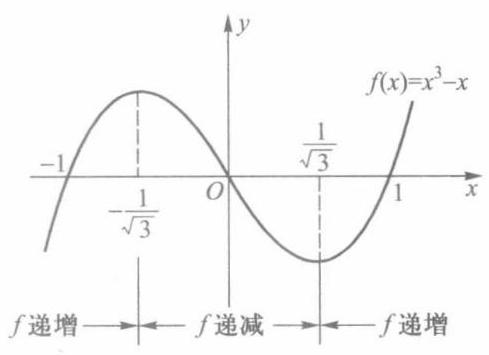
\includegraphics[width=.3\textwidth]{images/P035.jpg}
	\caption{图 $6-4$}
	\label{fig:P035}
\end{figure}

%定理 6.4
\begin{theorem}{严格递增 (递减) 的充要条件}{the:严格递增 (递减) 的充要条件}
若函数 \(f\) 在(a, b)上可导,则 \(f\) 在 (a, b)上严格递增 (递减) 的充要条件是:

(i) 对一切 \(x \in  \left( {a,b}\right)\) ,有 \({f}^{\prime }\left( x\right)  \geq  0\left( {{f}^{\prime }\left( x\right) }\right.\)  \(\leq  0)\) ；

(ii) 在(a, b)的任何子区间上 \({f}^{\prime }\left( x\right)  ≢ 0\) .
\end{theorem}


我们将这个定理的证明留给读者. 此定理有以下一个简单的推论.

%推论
\begin{corollary}{严格递增 (严格递减)}{pro:严格递增 (严格递减)}
设函数在区间 \(I\) 上可微,若 \({f}^{\prime }\left( x\right)  > 0\)  \(\left( {{f}^{\prime }\left( x\right)  < 0}\right)\) ,则 \(f\) 在 \(I\) 上严格递增 (严格递减).
\end{corollary}


%注
\begin{remark}
若 \(f\) 在(a, b)上 (严格) 递增 (减),且在点 \(a\) 右连续,则 \(f\) 在 \(\lbrack a,b)\) 上亦为 (严格) 递增 (减),对右端点 \(b\) 可类似讨论.

\end{remark}

%例 5
\begin{example}
证明不等式
\[
{\mathrm{e}}^{x} > 1 + x,x \neq  0.
\]
\end{example}

%证
\begin{proof}
设 \(f\left( x\right)  = {\mathrm{e}}^{x} - 1 - x\) ,则 \({f}^{\prime }\left( x\right)  = {\mathrm{e}}^{x} - 1\) . 故当 \(x > 0\) 时, \({f}^{\prime }\left( x\right)  > 0,f\) 严格递增; 当 \(x < 0\) , \({f}^{\prime }\left( x\right)  < 0,f\) 严格递减. 又由于 \(f\) 在点 \(x = 0\) 连续,则当 \(x \neq  0\) 时,
\[
f\left( x\right)  > f\left( 0\right)  = 0,
\]
从而证得
\[
{\mathrm{e}}^{x} > 1 + x,x \neq  0.
\]
\end{proof}

%定理 6.5
\begin{theorem}{达布 (Darboux) 定理}{the:达布 (Darboux) 定理}
若函数 \(f\) 在 \(\left\lbrack  {a,b}\right\rbrack\) 上可导,且 \({f}^{\prime }{}_{ + }\left( a\right)  \neq  {f}^{\prime }{}_{ - }\left( b\right) ,k\) 为介于 \({f}_{ + }^{\prime }\left( a\right) ,{f}_{ - }^{\prime }\left( b\right)\) 之间任一实数,则至少存在一点 \(\xi  \in  \left( {a,b}\right)\) ,使得
\[
{f}^{\prime }\left( \xi \right)  = k.
\]
\end{theorem}

%证
\begin{proof}
设 \(F\left( x\right)  = f\left( x\right)  - {kx}\) ,则 \(F\left( x\right)\) 在 \(\left\lbrack  {a,b}\right\rbrack\) 上可导,且
\[
{F}_{ + }^{\prime }\left( a\right)  \cdot  {F}_{ - }^{\prime }\left( b\right)  = \left( {{f}_{ + }^{\prime }\left( a\right)  - k}\right) \left( {{f}_{ - }^{\prime }\left( b\right)  - k}\right)  < 0.
\]
不妨设 \({F}_{ + }^{\prime }\left( a\right)  > 0,{F}_{ - }^{\prime }\left( b\right)  < 0\) . 由第五章 §1 例 8,分别存在 \({x}_{1} \in  {U}_{ + }^{ \circ  }\left( a\right) ,{x}_{2} \in  {U}_{ - }^{ \circ  }\left( b\right)\) ,且 \({x}_{1}\)  \(< {x}_{2}\) ,使得
\[
F\left( {x}_{1}\right)  > F\left( a\right) ,\;F\left( {x}_{2}\right)  > F\left( b\right) . \tag{8}
\]
因为 \(F\) 在 \(\left\lbrack  {a,b}\right\rbrack\) 上可导,所以连续. 根据最大、最小值定理 (定理 4.6),存在一点 \(\xi  \in  \left\lbrack  {a,b}\right\rbrack\) ,使 \(F\) 在点 \(\xi\) 取得最大值. 由 (8) 式,可知 \(\xi  \neq  a,b\) . 这就说明 \(\xi\) 是 \(F\) 的极大值点. 由费马定理得 \({F}^{\prime }\left( \xi \right)  = 0\) ,即
\[
{f}^{\prime }\left( \xi \right)  = k,\;\xi  \in  \left( {a,b}\right) .
\]
\end{proof}

有时称上述定理为导函数的介值定理.

%推论
\begin{corollary}{严格单调}{pro:严格单调}
设函数 \(f\left( x\right)\) 在区间 \(I\) 上满足 \({f}^{\prime }\left( x\right)  \neq  0\) ,那么 \(f\left( x\right)\) 在区间 \(I\) 上严格单调.
\end{corollary}


\subsection{习题 6.1}

1. 试讨论下列函数在指定区间上是否存在一点 \(\xi\) ,使 \({f}^{\prime }\left( \xi \right)  = 0\) :

(1) \(f\left( x\right)  = \left\{  \begin{array}{ll} x\sin \frac{1}{x}, & 0 < x \leq  \frac{1}{\pi }, \\  0, & x = 0; \end{array}\right.\)

(2) \(f\left( x\right)  = \left| x\right| , - 1 \leq  x \leq  1\) .

2. 证明:

(1) 方程 \({x}^{3} - {3x} + c = 0\) (这里 \(c\) 为常数) 在区间 \(\left\lbrack  {0,1}\right\rbrack\) 上不可能有两个不同的实根；

(2)方程 \({x}^{n} + {px} + q = 0\) ( \(n\) 为正整数, \(p\) , \(q\) 为实数)当 \(n\) 为偶数时至多有两个实根,当 \(n\) 为奇数时至多有三个实根.

3. 证明定理 6.2 的推论 2 .

4. 证明:

(1) 若函数 \(f\) 在 \(\left\lbrack  {a,b}\right\rbrack\) 上可导,且 \({f}^{\prime }\left( x\right)  \geq  m\) ,则
\[
f\left( b\right)  \geq  f\left( a\right)  + m\left( {b - a}\right) ;
\]

(2)若函数 \(f\) 在 \(\left\lbrack  {a,b}\right\rbrack\) 上可导,且 \(\left| {{f}^{\prime }\left( x\right) }\right|  \leq  M\) ,则
\[
\left| {f\left( b\right)  - f\left( a\right) }\right|  \leq  M\left( {b - a}\right) ;
\]

(3)对任意实数 \({x}_{1},{x}_{2}\) ,都有 \(\left| {\sin {x}_{1} - \sin {x}_{2}}\right|  \leq  \left| {{x}_{1} - {x}_{2}}\right|\) .

5. 应用拉格朗日中值定理证明下列不等式:

(1) \(\frac{b - a}{b} < \ln \frac{b}{a} < \frac{b - a}{a}\) ,其中 \(0 < a < b\) ；

(2) \(\frac{h}{1 + {h}^{2}} < \arctan h < h\) ,其中 \(h > 0\) .

6. 确定下列函数的单调区间:

(1) \(f\left( x\right)  = {3x} - {x}^{2}\) ;

(2) \(f\left( x\right)  = 2{x}^{2} - \ln x\) ;

(3) \(f\left( x\right)  = \sqrt{{2x} - {x}^{2}}\) ;

(4) \(f\left( x\right)  = \frac{{x}^{2} - 1}{x}\) .

7. 应用函数的单调性证明下列不等式:

(1) \(\tan x > x - \frac{{x}^{3}}{3},x \in  \left( {0,\frac{\pi }{2}}\right)\) ;

(2) \(\frac{2x}{\pi } < \sin x < x,x \in  \left( {0,\frac{\pi }{2}}\right)\) ；

(3) \(x - \frac{{x}^{2}}{2} < \ln \left( {1 + x}\right)  < x - \frac{{x}^{2}}{2\left( {1 + x}\right) },x > 0\) .

8. 以 \(S\left( x\right)\) 记由 \(\left( {a,f\left( a\right) }\right) ,\left( {b,f\left( b\right) }\right) ,\left( {x,f\left( x\right) }\right)\) 三点组成的三角形面积,试对 \(S\left( x\right)\) 应用罗尔中值定理证明拉格朗日中值定理.

9. 设 \(f\) 为 \(\left\lbrack  {a,b}\right\rbrack\) 上二阶可导函数, \(f\left( a\right)  = f\left( b\right)  = 0\) ,并存在一点 \(c \in  \left( {a,b}\right)\) ,使得 \(f\left( c\right)  > 0\) . 证明至少存在一点 \(\xi  \in  \left( {a,b}\right)\) ,使得 \({f}^{\prime \prime }\left( \xi \right)  < 0\) .

10. 设函数 \(f\) 在(a, b)上可导,且 \({f}^{\prime }\) 单调. 证明 \({f}^{\prime }\) 在(a, b)上连续.

11. 设 \(p\left( x\right)\) 为多项式, \(\alpha\) 为 \(p\left( x\right)  = 0\) 的 \(r\) 重实根. 证明 \(\alpha\) 必定是 \({p}^{\prime }\left( x\right)  = 0\) 的 \(r - 1\) 重实根.

12. 证明: 设 \(f\) 为 \(n\) 阶可导函数,若方程 \(f\left( x\right)  = 0\) 有 \(n + 1\) 个相异的实根,则方程 \({f}^{\left( n\right) }\left( x\right)  = 0\) 至少有一个实根.

13. 设 \(a > 0\) . 证明函数 \(f\left( x\right)  = {x}^{3} + {ax} + b\) 存在唯一的零点.

14. 证明: \(\frac{\tan x}{x} > \frac{x}{\sin x},x \in  \left( {0,\frac{\pi }{2}}\right)\) .

15. 证明: 若函数 \(f,g\) 在区间 \(\left\lbrack  {a,b}\right\rbrack\) 上可导,且 \({f}^{\prime }\left( x\right)  > {g}^{\prime }\left( x\right) ,f\left( a\right)  = g\left( a\right)\) ,则在 \((a,b\rbrack\) 上有 \(f\left( x\right)  >\)  \(g\left( x\right)\) .

\section{柯西中值定理和不定式极限}

\subsection{柯西中值定理}

现给出一个形式更一般的微分中值定理.

%定理 6.6
\begin{theorem}{柯西中值定理}{the:柯西中值定理}
设函数 \(f\) 和 \(g\) 满足:

(i) 在 \(\left\lbrack  {a,b}\right\rbrack\) 上都连续;

(ii) 在(a, b)上都可导;

(iii) \({f}^{\prime }\left( x\right)\) 和 \({g}^{\prime }\left( x\right)\) 不同时为零;

(iv) \(g\left( a\right)  \neq  g\left( b\right)\) ,

则存在 \(\xi  \in  \left( {a,b}\right)\) ,使得
\[
\frac{{f}^{\prime }\left( \xi \right) }{{g}^{\prime }\left( \xi \right) } = \frac{f\left( b\right)  - f\left( a\right) }{g\left( b\right)  - g\left( a\right) }. \tag{1}
\]
\end{theorem}

%证
\begin{proof}
作辅助函数
\[
F\left( x\right)  = f\left( x\right)  - f\left( a\right)  - \frac{f\left( b\right)  - f\left( a\right) }{g\left( b\right)  - g\left( a\right) }\left( {g\left( x\right)  - g\left( a\right) }\right) .
\]
易见 \(F\) 在 \(\left\lbrack  {a,b}\right\rbrack\) 上满足罗尔定理条件,故存在 \(\xi  \in  \left( {a,b}\right)\) ,使得
\[
{F}^{\prime }\left( \xi \right)  = {f}^{\prime }\left( \xi \right)  - \frac{f\left( b\right)  - f\left( a\right) }{g\left( b\right)  - g\left( a\right) }{g}^{\prime }\left( \xi \right)  = 0.
\]
因为 \({g}^{\prime }\left( \xi \right)  \neq  0\) (否则由上式 \({f}^{\prime }\left( \xi \right)\) 也为零),所以可把上式改写成 (1) 式.
\end{proof}


柯西中值定理有与前两个中值定理相类似的几何意义. 只是现在要把 \(f,g\) 这两个函数写作以 \(x\) 为参量的参量方程
\[
\left\{  \begin{array}{l} u = g\left( x\right) , \\  v = f\left( x\right) , \end{array}\right.
\]
它在 \({uOv}\) 平面上表示一段曲线 (图6-5). 由于 (1) 式右边的 \(\frac{f\left( b\right)  - f\left( a\right) }{g\left( b\right)  - g\left( a\right) }\) 表示连接该曲线两端的弦 \({AB}\) 的斜率,而 (1) 式左边的
\[
\frac{{f}^{\prime }\left( \xi \right) }{{g}^{\prime }\left( \xi \right) } = {\left. \frac{\mathrm{d}v}{\mathrm{\;d}u}\right| }_{x = \xi }
\]
则表示该曲线上与 \(x = \xi\) 相对应的一点 \(C(g\left( \xi \right)\) , \(f\left( \xi \right) )\) 处的切线的斜率. 因此 (1) 式即表示上述切线与弦 \({AB}\) 互相平行.

\begin{figure}
    \centering
    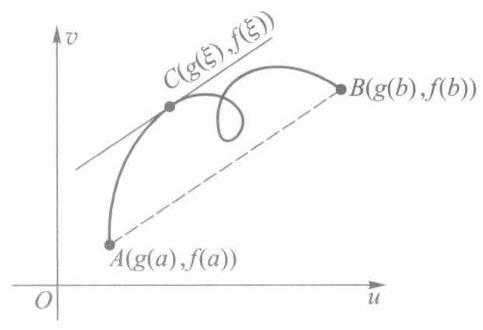
\includegraphics[width=.3\textwidth]{images/P036.jpg}
    \caption{图 $6-5$}
    \label{fig:P036}
\end{figure}

%例 1
\begin{example}
设函数 \(f\) 在 \(\left\lbrack  {a,b}\right\rbrack  \left( {a > 0}\right)\) 上连续,在(a, b)上可导,则存在 \(\xi  \in  \left( {a,b}\right)\) ,使得
\[
f\left( b\right)  - f\left( a\right)  = \xi {f}^{\prime }\left( \xi \right) \ln \frac{b}{a}. \tag{2}
\]
\end{example}

%证
\begin{proof}
设 \(g\left( x\right)  = \ln x\) ,显然它在 \(\left\lbrack  {a,b}\right\rbrack\) 上与 \(f\left( x\right)\) 一起满足柯西中值定理条件,于是存在 \(\xi  \in  \left( {a,b}\right)\) ,使得
\[
\frac{f\left( b\right)  - f\left( a\right) }{\ln b - \ln a} = \frac{{f}^{\prime }\left( \xi \right) }{\frac{1}{\xi }}.
\]
上式整理后便得到所要证明的 (2) 式.
\end{proof}


%例 2
\begin{example}
设 \(f\) 在区间 \((0,1\rbrack\) 上可导, \(\mathop{\lim }\limits_{{x \rightarrow  {0}^{ + }}}\sqrt{x}{f}^{\prime }\left( x\right)  = A\) . 证明: \(f\) 在区间 \((0,1\rbrack\) 上一致连续.
\end{example}


%证
\begin{proof}
设 \(M = \left| A\right|  + 1\) . 因为 \(\mathop{\lim }\limits_{{x \rightarrow  {0}^{ + }}}\sqrt{x}{f}^{\prime }\left( x\right)  = A\) ,所以存在 \({\delta }_{1}\left( {0 < {\delta }_{1} < 1}\right)\) ,当 \(0 < x < {\delta }_{1}\) 时, \(\left| {\sqrt{x}{f}^{\prime }\left( x\right) }\right|  < M\) . 那么对任意的 \(x,y \in  \left( {0,{\delta }_{1}}\right\rbrack  ,x < y\) ,由柯西中值定理,存在 \(\xi\) ,使
\[
\left| \frac{f\left( x\right)  - f\left( y\right) }{\sqrt{x} - \sqrt{y}}\right|  = 2\left| {\sqrt{\xi }{f}^{\prime }\left( \xi \right) }\right|  \leq  {2M},\;0 < x < \xi  < y \leq  {\delta }_{1}.
\]
由此
\[
\left| {f\left( x\right)  - f\left( y\right) }\right|  \leq  {2M}\left| {\sqrt{x} - \sqrt{y}}\right| .
\]
因为函数 \(\sqrt{x}\) 在区间 \(\left( {0,{\delta }_{1}}\right\rbrack\) 上一致连续,所以 \(f\left( x\right)\) 亦在 \(\left( {0,{\delta }_{1}}\right\rbrack\) 上一致连续. 又 \(f\left( x\right)\) 在 \(\left\lbrack  {{\delta }_{1},1}\right\rbrack\) 上连续,从而为一致连续,故函数 \(f\) 在区间 \((0,1\rbrack\) 上一致连续.
\end{proof}


\subsection{不定式极限}

我们在第三章学习无穷小 (大) 量阶的比较时, 已经遇到过两个无穷小 (大) 量之比的极限. 由于这种极限可能存在, 也可能不存在, 因此我们把两个无穷小量或两个无穷大量之比的极限统称为不定式极限,分别记为 \(\frac{0}{0}\) 型或 \(\frac{\infty }{\infty }\) 型的不定式极限. 现在我们将以导数为工具研究不定式极限, 这个方法通常称为洛必达 ( L'Hospital ) 法则. 柯西中值定理则是建立洛必达法则的理论依据.

1. \(\frac{0}{0}\) 型不定式极限

%定理 6.7
\begin{theorem}{}{the:6.7}
若函数 \(f\) 和 \(g\) 满足:

(i) \(\mathop{\lim }\limits_{{x \rightarrow  {x}_{0}}}f\left( x\right)  = \mathop{\lim }\limits_{{x \rightarrow  {x}_{0}}}g\left( x\right)  = 0\) ;

(ii) 在点 \({x}_{0}\) 的某空心邻域 \({U}^{ \circ  }\left( {x}_{0}\right)\) 上两者都可导,且 \({g}^{\prime }\left( x\right)  \neq  0\) ;

(iii) \(\mathop{\lim }\limits_{{x \rightarrow  {x}_{0}}}\frac{{f}^{\prime }\left( x\right) }{{g}^{\prime }\left( x\right) } = A\left( {A\text{ 可为实数,也可为 } \pm  \infty \text{ 或 }\infty }\right)\) ,

则
\[
\mathop{\lim }\limits_{{x \rightarrow  {x}_{0}}}\frac{f\left( x\right) }{g\left( x\right) } = \mathop{\lim }\limits_{{x \rightarrow  {x}_{0}}}\frac{{f}^{\prime }\left( x\right) }{{g}^{\prime }\left( x\right) } = A.
\]
\end{theorem}

%证
\begin{proof}
补充定义 \(f\left( {x}_{0}\right)  = g\left( {x}_{0}\right)  = 0\) ,使得 \(f\) 与 \(g\) 在点 \({x}_{0}\) 连续. 任取 \(x \in  {U}^{ \circ  }\left( {x}_{0}\right)\) ,在区间 \(\left\lbrack  {{x}_{0},x}\right\rbrack  \left( {\text{ 或 }\left\lbrack  {x,{x}_{0}}\right\rbrack  }\right)\) 上应用柯西中值定理,有
\[
\frac{f\left( x\right)  - f\left( {x}_{0}\right) }{g\left( x\right)  - g\left( {x}_{0}\right) } = \frac{{f}^{\prime }\left( \xi \right) }{{g}^{\prime }\left( \xi \right) },
\]
即
\[
\frac{f\left( x\right) }{g\left( x\right) } = \frac{{f}^{\prime }\left( \xi \right) }{{g}^{\prime }\left( \xi \right) }\;\left( {\xi \text{ 介于 }{x}_{0}\text{ 与 }x\text{ 之间 }}\right) .
\]
当令 \(x \rightarrow  {x}_{0}\) 时,也有 \(\xi  \rightarrow  {x}_{0}\) ,故得
\[
\mathop{\lim }\limits_{{x \rightarrow  {x}_{0}}}\frac{f\left( x\right) }{g\left( x\right) } = \mathop{\lim }\limits_{{x \rightarrow  {x}_{0}}}\frac{{f}^{\prime }\left( \xi \right) }{{g}^{\prime }\left( \xi \right) } = \mathop{\lim }\limits_{{x \rightarrow  {x}_{0}}}\frac{{f}^{\prime }\left( x\right) }{{g}^{\prime }\left( x\right) } = A.
\]
\end{proof}

注意 若将定理 6.7 中 \(x \rightarrow  {x}_{0}\) 换成 \(x \rightarrow  {x}_{0}^{ + },x \rightarrow  {x}_{0}^{ - },x \rightarrow   \pm  \infty ,x \rightarrow  \infty\) ,只要相应地修正条件 (ii) 中的邻域, 也可得到同样的结论.

%例 3
\begin{example}
求 \(\mathop{\lim }\limits_{{x \rightarrow  \pi }}\frac{1 + \cos x}{{\tan }^{2}x}\) .
\end{example}


%解
\begin{solution}
容易检验 \(f\left( x\right)  = 1 + \cos x\) 与 \(g\left( x\right)  = {\tan }^{2}x\) 在点 \({x}_{0} = \pi\) 的邻域上满足定理 6.7 的条件 (i) 和 (ii) , 又因
\[
\mathop{\lim }\limits_{{x \rightarrow  \pi }}\frac{{f}^{\prime }\left( x\right) }{{g}^{\prime }\left( x\right) } = \mathop{\lim }\limits_{{x \rightarrow  \pi }}\frac{-\sin x}{2\tan x{\sec }^{2}x} =  - \mathop{\lim }\limits_{{x \rightarrow  \pi }}\frac{{\cos }^{3}x}{2} = \frac{1}{2},
\]
故由洛必达法则求得
\[
\mathop{\lim }\limits_{{x \rightarrow  \pi }}\frac{f\left( x\right) }{g\left( x\right) } = \mathop{\lim }\limits_{{x \rightarrow  \pi }}\frac{{f}^{\prime }\left( x\right) }{{g}^{\prime }\left( x\right) } = \frac{1}{2}.
\]
\end{solution}

如果 \(\mathop{\lim }\limits_{{x \rightarrow  {x}_{0}}}\frac{{f}^{\prime }\left( x\right) }{{g}^{\prime }\left( x\right) }\) 仍是 \(\frac{0}{0}\) 型不定式极限,只要有可能,我们可再次用洛必达法则,即考察极限 \(\mathop{\lim }\limits_{{x \rightarrow  {x}_{0}}}\frac{{f}^{\prime }\left( x\right) }{{g}^{\prime }\left( x\right) }\) 是否存在. 当然这时 \({f}^{\prime }\) 和 \({g}^{\prime }\) 在点 \({x}_{0}\) 的某邻域上必须满足定理 6.7 的条件.

%例 4
\begin{example}
求 \(\mathop{\lim }\limits_{{x \rightarrow  0}}\frac{{\mathrm{e}}^{x} - {\left( 1 + 2x\right) }^{\frac{1}{2}}}{\ln \left( {1 + {x}^{2}}\right) }\) .
\end{example}


%解
\begin{solution}
利用 \(\ln \left( {1 + {x}^{2}}\right)  \sim  {x}^{2}\left( {x \rightarrow  0}\right)\) ,则得
\[
\mathop{\lim }\limits_{{x \rightarrow  0}}\frac{{\mathrm{e}}^{x} - {\left( 1 + 2x\right) }^{\frac{1}{2}}}{\ln \left( {1 + {x}^{2}}\right) } = \mathop{\lim }\limits_{{x \rightarrow  0}}\frac{{\mathrm{e}}^{x} - {\left( 1 + 2x\right) }^{\frac{1}{2}}}{{x}^{2}} = \mathop{\lim }\limits_{{x \rightarrow  0}}\frac{{\mathrm{e}}^{x} - {\left( 1 + 2x\right) }^{-\frac{1}{2}}}{2x}
\]
\[
= \mathop{\lim }\limits_{{x \rightarrow  0}}\frac{{\mathrm{e}}^{x} + {\left( 1 + 2x\right) }^{-\frac{3}{2}}}{2} = \frac{2}{2} = 1.
\]
\end{solution}

%例 5
\begin{example}
求 \(\mathop{\lim }\limits_{{x \rightarrow  {0}^{ + }}}\frac{\sqrt{x}}{1 - {\mathrm{e}}^{\sqrt{x}}}\) .
\end{example}


%解
\begin{solution}
这是 \(\frac{0}{0}\) 型不定式极限,可直接运用洛必达法则求解. 但若作适当变换,在计算上可方便些. 为此,令 \(t = \sqrt{x}\) ,当 \(x \rightarrow  {0}^{ + }\) 时有 \(t \rightarrow  {0}^{ + }\) ,于是有
\[
\mathop{\lim }\limits_{{x \rightarrow  {0}^{ + }}}\frac{\sqrt{x}}{1 - {\mathrm{e}}^{\sqrt{x}}} = \mathop{\lim }\limits_{{t \rightarrow  {0}^{ + }}}\frac{t}{1 - {\mathrm{e}}^{t}} = \mathop{\lim }\limits_{{t \rightarrow  {0}^{ + }}}\frac{1}{-{\mathrm{e}}^{t}} =  - 1.
\]
\end{solution}

2. \(\frac{ \bullet  }{\infty }\) 型不定式极限

%定理 6.8
\begin{theorem}{}{the:6.8}
若函数 \(f\) 和 \(g\) 满足:

(i) 在 \({x}_{0}\) 的某个右邻域 \({U}_{ + }^{ \circ  }\left( {x}_{0}\right)\) 上两者可导,且 \({g}^{\prime }\left( x\right)  \neq  0\) ;

(ii) \(\mathop{\lim }\limits_{{x \rightarrow  {x}_{0}^{ + }}}g\left( x\right)  = \infty\) ;

(iii) \(\mathop{\lim }\limits_{{x \rightarrow  {x}_{0}^{ + }}}\frac{{f}^{\prime }\left( x\right) }{{g}^{\prime }\left( x\right) } = A\left( {A\text{ 可为实数,也可为 } \pm  \infty ,\infty }\right)\) ,

则
\[
\mathop{\lim }\limits_{{x \rightarrow  {x}_{0}^{ + }}}\frac{f\left( x\right) }{g\left( x\right) } = A.
\]
\end{theorem}

%证
\begin{proof}
先设 \(A\) 为实数,由 (iii),对任意正数 \(\varepsilon\) ,存在 \({x}_{1} \in  {U}_{ + }^{ \circ  }\left( {x}_{0}\right)\) ,对满足不等式 \({x}_{0} < x <\)  \({x}_{1}\) 的每一个 \(x\) ,有
\[
A - \frac{\varepsilon }{2} < \frac{{f}^{\prime }\left( x\right) }{{g}^{\prime }\left( x\right) } < A + \frac{\varepsilon }{2}, \tag{3}
\]
由条件 (ii), \(f\) 和 \(g\) 在区间 \(\left\lbrack  {x,{x}_{1}}\right\rbrack\) 上满足柯西中值定理,故存在 \(\xi  \in  \left( {x,{x}_{1}}\right)  \subset  \left( {{x}_{0},{x}_{1}}\right)\) , 使得
\[
A - \frac{\varepsilon }{2} < \left( {\frac{f\left( x\right) }{g\left( x\right) } - \frac{f\left( {x}_{1}\right) }{g\left( x\right) }}\right) \left( \frac{g\left( x\right) }{g\left( x\right)  - g\left( {x}_{1}\right) }\right)  = \frac{f\left( x\right)  - f\left( {x}_{1}\right) }{g\left( x\right)  - g\left( {x}_{1}\right) } = \frac{{f}^{\prime }\left( \xi \right) }{{g}^{\prime }\left( \xi \right) } < A + \frac{\varepsilon }{2}.
\]
(4)

因为 \(\mathop{\lim }\limits_{{x \rightarrow  {x}_{0}^{ + }}}\frac{g\left( x\right) }{g\left( x\right)  - g\left( {x}_{1}\right) } = 1\) ,所以由保号性,存在正数 \({\delta }_{1}\left( { < {x}_{1} - {x}_{0}}\right)\) ,使得当 \({x}_{0} < x < {x}_{0} + {\delta }_{1}\) 时, \(\frac{g\left( x\right) }{g\left( x\right)  - g\left( {x}_{1}\right) } > 0\) ,再根据 (4) 式可得
\[
\left( {1 - \frac{g\left( {x}_{1}\right) }{g\left( x\right) }}\right) \left( {A - \frac{\varepsilon }{2}}\right)  + \frac{f\left( {x}_{1}\right) }{g\left( x\right) } < \frac{f\left( x\right) }{g\left( x\right) } < \left( {1 - \frac{g\left( {x}_{1}\right) }{g\left( x\right) }}\right) \left( {A + \frac{\varepsilon }{2}}\right)  + \frac{f\left( {x}_{1}\right) }{g\left( x\right) }. \tag{5}
\]
又因为 \(\mathop{\lim }\limits_{{x \rightarrow  {x}_{0}^{ + }}}g\left( x\right)  = \infty\) ,所以
\[
\mathop{\lim }\limits_{{x \rightarrow  {x}_{0}^{ + }}}\left( {\left( {1 - \frac{g\left( {x}_{1}\right) }{g\left( x\right) }}\right) \left( {A - \frac{\varepsilon }{2}}\right)  + \frac{f\left( {x}_{1}\right) }{g\left( x\right) }}\right)  = A - \frac{\varepsilon }{2},
\]
\[
\mathop{\lim }\limits_{{x \rightarrow  {x}_{0}^{ + }}}\left( {\left( {1 - \frac{g\left( {x}_{1}\right) }{g\left( x\right) }}\right) \left( {A + \frac{\varepsilon }{2}}\right)  + \frac{f\left( {x}_{1}\right) }{g\left( x\right) }}\right)  = A + \frac{\varepsilon }{2}.
\]
再由保号性得知: 存在正数 \(\delta \left( { < {\delta }_{1}}\right)\) ,当 \({x}_{0} < x < {x}_{0} + \delta\) 时,有
\[
A - \varepsilon  < \frac{f\left( x\right) }{g\left( x\right) } < A + \varepsilon ,
\]
这样就证明了
\[
\mathop{\lim }\limits_{{x \rightarrow  {x}_{0}^{ + }}}\frac{f\left( x\right) }{g\left( x\right) } = A.
\]
类似地可以证明当 \(A =  \pm  \infty\) 或 \(\infty\) 的情形,这里就不再赘述了.
\end{proof}


定理 6.8 对于 \(x \rightarrow  {x}_{0}^{ - },x \rightarrow  {x}_{0}\) 或 \(x \rightarrow   \pm  \infty ,x \rightarrow  \infty\) 等情形也有相同的结论.

如果 \({f}^{\prime },{g}^{\prime },{f}^{\prime \prime },{g}^{\prime \prime }\) 满足相应条件,我们可以再次应用定理 6.8.

%例 6
\begin{example}
求 \(\mathop{\lim }\limits_{{x \rightarrow   + \infty }}\frac{\ln x}{x}\) .
\end{example}


%解
\begin{solution}
由定理 6.8 , 有
\[
\mathop{\lim }\limits_{{x \rightarrow   + \infty }}\frac{\ln x}{x} = \mathop{\lim }\limits_{{x \rightarrow   + \infty }}\frac{{\left( \ln x\right) }^{\prime }}{{\left( x\right) }^{\prime }} = \mathop{\lim }\limits_{{x \rightarrow   + \infty }}\frac{1}{x} = 0.
\]
\end{solution}

%例 7
\begin{example}
求 \(\mathop{\lim }\limits_{{x \rightarrow   + \infty }}\frac{{\mathrm{e}}^{x}}{{x}^{3}}\) .
\end{example}


%解
\begin{solution}
\(\mathop{\lim }\limits_{{x \rightarrow   + \infty }}\frac{{\mathrm{e}}^{x}}{{x}^{3}} = \mathop{\lim }\limits_{{x \rightarrow   + \infty }}\frac{{\mathrm{e}}^{x}}{3{x}^{2}} = \mathop{\lim }\limits_{{x \rightarrow   + \infty }}\frac{{\mathrm{e}}^{x}}{6x} = \mathop{\lim }\limits_{{x \rightarrow   + \infty }}\frac{{\mathrm{e}}^{x}}{6} =  + \infty\) .
\end{solution}


%例 8
\begin{example}
设 \(f\left( x\right)\) 在区间 \(\lbrack 0, + \infty )\) 上可导, \(\mathop{\lim }\limits_{{x \rightarrow   + \infty }}\left\lbrack  {f\left( x\right)  + {f}^{\prime }\left( x\right) }\right\rbrack   = A\) . 证明: \(\mathop{\lim }\limits_{{x \rightarrow   + \infty }}f\left( x\right)  = A\) .
\end{example}


%证
\begin{proof}
因为 \(\mathop{\lim }\limits_{{x \rightarrow   + \infty }}{\mathrm{e}}^{x} =  + \infty\) ,所以由定理 6.8 得
\[
\mathop{\lim }\limits_{{x \rightarrow   + \infty }}f\left( x\right)  = \mathop{\lim }\limits_{{x \rightarrow   + \infty }}\frac{{\mathrm{e}}^{x}f\left( x\right) }{{\mathrm{e}}^{x}} = \mathop{\lim }\limits_{{x \rightarrow   + \infty }}\frac{{\mathrm{e}}^{x}\left\lbrack  {f\left( x\right)  + {f}^{\prime }\left( x\right) }\right\rbrack  }{{\mathrm{e}}^{x}} = \mathop{\lim }\limits_{{x \rightarrow   + \infty }}\left\lbrack  {f\left( x\right)  + {f}^{\prime }\left( x\right) }\right\rbrack   = A.
\]
\end{proof}

%注
\begin{remark}
1 若 \(\mathop{\lim }\limits_{{x \rightarrow  {x}_{0}}}\frac{{f}^{\prime }\left( x\right) }{{g}^{\prime }\left( x\right) }\) 不存在,并不能说明 \(\mathop{\lim }\limits_{{x \rightarrow  {x}_{0}}}\frac{f\left( x\right) }{g\left( x\right) }\) 不存在. (试想,这是为什么?)

\end{remark}

%注
\begin{remark}
2 不能对任何比式极限都按洛必达法则求解. 首先必须注意它是不是不定式极限, 其次是否满足洛必达法则的其他条件.
\end{remark}

下面这个简单的极限
\[
\mathop{\lim }\limits_{{x \rightarrow  \infty }}\frac{x + \sin x}{x} = 1
\]
虽然是 \(\frac{\infty }{\infty }\) 型,但若不顾条件随便使用洛必达法则:
\[
\mathop{\lim }\limits_{{x \rightarrow   + \infty }}\frac{x + \sin x}{x} = \mathop{\lim }\limits_{{x \rightarrow   + \infty }}\frac{1 + \cos x}{1},
\]
就会因右式的极限不存在而推出原极限不存在的错误结论.

3. 其他类型不定式极限

不定式极限还有 \(0 \cdot  \infty ,{1}^{\infty },{0}^{0},{\infty }^{0},\infty  - \infty\) 等类型. 经过简单变换,它们一般均可化为 \(\frac{0}{0}\) 型或 \(\frac{\infty }{\infty }\) 型的极限.

%例 9
\begin{example}
求 \(\mathop{\lim }\limits_{{x \rightarrow  {0}^{ + }}}x\ln x\) .
\end{example}


%解
\begin{solution}
这是一个 \(0 \cdot  \infty\) 型不定式极限. 用恒等变形 \(x\ln x = \frac{\ln x}{\frac{1}{x}}\) 将它转化为 \(\frac{\infty }{\infty }\) 型的不定式极限, 并应用洛必达法则得到
\[
\mathop{\lim }\limits_{{x \rightarrow  {0}^{ + }}}x\ln x = \mathop{\lim }\limits_{{x \rightarrow  {0}^{ + }}}\frac{\ln x}{\frac{1}{x}} = \mathop{\lim }\limits_{{x \rightarrow  {0}^{ + }}}\frac{\frac{1}{x}}{-\frac{1}{{x}^{2}}} = \mathop{\lim }\limits_{{x \rightarrow  {0}^{ + }}}\left( {-x}\right)  = 0.
\]
\end{solution}

%例 10
\begin{example}
求 \(\mathop{\lim }\limits_{{x \rightarrow  0}}{\left( \cos x\right) }^{\frac{1}{{x}^{2}}}\) .
\end{example}


%解
\begin{solution}
这是一个 \({1}^{\infty }\) 型不定式极限. 作恒等变形
\[
{\left( \cos x\right) }^{\frac{1}{{x}^{2}}} = {\mathrm{e}}^{\frac{1}{{x}^{2}}\ln \cos x},
\]
其指数部分的极限 \(\mathop{\lim }\limits_{{x \rightarrow  0}}\frac{1}{{x}^{2}}\ln \cos x\) 是 \(\frac{0}{0}\) 型不定式极限,可先求得
\[
\mathop{\lim }\limits_{{x \rightarrow  0}}\frac{\ln \cos x}{{x}^{2}} = \mathop{\lim }\limits_{{x \rightarrow  0}}\frac{-\tan x}{2x} =  - \frac{1}{2},
\]
从而得到
\[
\mathop{\lim }\limits_{{x \rightarrow  0}}{\left( \cos x\right) }^{\frac{1}{{x}^{2}}} = {\mathrm{e}}^{-\frac{1}{2}}.
\]
\end{solution}

%例 11
\begin{example}
求 \(\mathop{\lim }\limits_{{x \rightarrow  {0}^{ + }}}{\left( \sin x\right) }^{\frac{k}{1 + \ln x}}\;\left( {k\text{ 为常数 }}\right)\) .
\end{example}


%解
\begin{solution}
这是一个 \({0}^{ \circ  }\) 型不定式极限,按上例变形的方法,先求 \(\frac{\infty }{\infty }\) 型极限:
\[
\mathop{\lim }\limits_{{x \rightarrow  {0}^{ + }}}\frac{k\ln \sin x}{1 + \ln x} = \mathop{\lim }\limits_{{x \rightarrow  {0}^{ + }}}\frac{\frac{k\cos x}{\sin x}}{\frac{1}{x}} = \mathop{\lim }\limits_{{x \rightarrow  {0}^{ + }}}k\cos x \cdot  \frac{x}{\sin x} = k,
\]
然后得到
\[
\mathop{\lim }\limits_{{x \rightarrow  {0}^{ + }}}{\left( \sin x\right) }^{\frac{k}{1 + \ln x}} = {\mathrm{e}}^{k}\;\left( {k \neq  0}\right) .
\]
当 \(k = 0\) 时上面所得的结果显然成立.
\end{solution}


%例 12
\begin{example}
求 \(\mathop{\lim }\limits_{{x \rightarrow   + \infty }}{\left( x + \sqrt{1 + {x}^{2}}\right) }^{\frac{1}{\ln x}}\) .
\end{example}


%解
\begin{solution}
这是一个 \({\infty }^{0}\) 型不定式极限. 类似地先求其对数的极限 \(\left( {\frac{\infty }{\infty }\text{ 型 }}\right)\) :
\[
\mathop{\lim }\limits_{{x \rightarrow   + \infty }}\frac{\ln \left( {x + \sqrt{1 + {x}^{2}}}\right) }{\ln x} = \mathop{\lim }\limits_{{x \rightarrow   + \infty }}\frac{\frac{1}{\sqrt{1 + {x}^{2}}}}{\frac{1}{x}} = 1,
\]
于是有
\[
\mathop{\lim }\limits_{{x \rightarrow   + \infty }}{\left( x + \sqrt{1 + {x}^{2}}\right) }^{\frac{1}{\ln x}} = \mathrm{e}.
\]
\end{solution}

%例 13
\begin{example}
求 \(\mathop{\lim }\limits_{{x \rightarrow  1}}\left( {\frac{1}{x - 1} - \frac{1}{\ln x}}\right)\) .
\end{example}


%解
\begin{solution}
这是一个 \(\infty  - \infty\) 型不定式极限,通分后化为 \(\frac{0}{0}\) 型的极限,即
\[
\mathop{\lim }\limits_{{x \rightarrow  1}}\left( {\frac{1}{x - 1} - \frac{1}{\ln x}}\right)  = \mathop{\lim }\limits_{{x \rightarrow  1}}\frac{\ln x - x + 1}{\left( {x - 1}\right) \ln x} = \mathop{\lim }\limits_{{x \rightarrow  1}}\frac{\frac{1}{x} - 1}{\frac{x - 1}{x} + \ln x}
\]
\[
= \mathop{\lim }\limits_{{x \rightarrow  1}}\frac{1 - x}{x - 1 + x\ln x} = \mathop{\lim }\limits_{{x \rightarrow  1}}\frac{-1}{2 + \ln x} =  - \frac{1}{2}\text{ . }
\]
\end{solution}

%例 14
\begin{example}
设
\[
f\left( x\right)  = \left\{  \begin{array}{ll} \frac{g\left( x\right) }{x}, & x \neq  0, \\  0, & x = 0, \end{array}\right.
\]
且已知 \(g\left( 0\right)  = {g}^{\prime }\left( 0\right)  = 0,{g}^{\prime \prime }\left( 0\right)  = 3\) ,试求 \({f}^{\prime }\left( 0\right)\) .
\end{example}


%解
\begin{solution}
因为
\[
\frac{f\left( x\right)  - f\left( 0\right) }{x - 0} = \frac{g\left( x\right) }{{x}^{2}},
\]
所以由洛必达法则得
\[
{f}^{\prime }\left( 0\right)  = \mathop{\lim }\limits_{{x \rightarrow  0}}\frac{g\left( x\right) }{{x}^{2}} = \mathop{\lim }\limits_{{x \rightarrow  0}}\frac{{g}^{\prime }\left( x\right) }{2x}
\]
\[
= \frac{1}{2}\mathop{\lim }\limits_{{x \rightarrow  0}}\frac{{g}^{\prime }\left( x\right)  - {g}^{\prime }\left( 0\right) }{x - 0} = \frac{1}{2}{g}^{\prime \prime }\left( 0\right)  = \frac{3}{2}.
\]
\end{solution}

问题两则:

(1)上例解法中,已知条件 \(g\left( 0\right)  = 0\) 用在何处？

(2)如果用两次洛必达法则, 得到
\[
{f}^{\prime }\left( 0\right)  = \cdots  = \mathop{\lim }\limits_{{x \rightarrow  0}}\frac{{g}^{\prime }\left( x\right) }{2x}
\]
\[
= \mathop{\lim }\limits_{{x \rightarrow  0}}\frac{{g}^{\prime \prime }\left( x\right) }{2} = \frac{1}{2}{g}^{\prime \prime }\left( 0\right)  = \frac{3}{2}\text{ . }
\]
错在何处?

最后指出, 对于数列的不定式极限, 可利用函数极限的归结原则, 通过先求相应形式的函数极限而得到结果.

%例 15
\begin{example}
求数列极限 \(\mathop{\lim }\limits_{{n \rightarrow  \infty }}{\left( 1 + \frac{1}{n} + \frac{1}{{n}^{2}}\right) }^{n}\) .

\end{example}

%解
\begin{solution}
先求函数极限 \(\mathop{\lim }\limits_{{x \rightarrow   + \infty }}{\left( 1 + \frac{1}{x} + \frac{1}{{x}^{2}}\right) }^{x}\left( {1{^\circ}\text{ 型 }}\right)\) . 类似于例 10,取对数后的极限为
\[
\mathop{\lim }\limits_{{x \rightarrow   + \infty }}x\ln \left( {1 + \frac{1}{x} + \frac{1}{{x}^{2}}}\right)  = \mathop{\lim }\limits_{{x \rightarrow   + \infty }}\frac{\ln \left( {1 + x + {x}^{2}}\right)  - \ln {x}^{2}}{\frac{1}{x}}
\]
\[
= \mathop{\lim }\limits_{{x \rightarrow   + \infty }}\frac{\frac{{2x} + 1}{1 + x + {x}^{2}} - \frac{2}{x}}{-\frac{1}{{x}^{2}}} = \mathop{\lim }\limits_{{x \rightarrow   + \infty }}\frac{{x}^{2} + {2x}}{{x}^{2} + x + 1} = 1,
\]
所以由归结原则可得
\[
\mathop{\lim }\limits_{{n \rightarrow  \infty }}{\left( 1 + \frac{1}{n} + \frac{1}{{n}^{2}}\right) }^{n} = \mathop{\lim }\limits_{{x \rightarrow   + \infty }}{\left( 1 + \frac{1}{x} + \frac{1}{{x}^{2}}\right) }^{x} = \mathrm{e}.
\]
\end{solution}

注意 不能在数列形式下直接用洛必达法则,因为对离散变量 \(n \in  {\mathbf{N}}_{ + }\) 求导数是没有意义的.

\subsection{习题 6.2}

1. 试问函数 \(f\left( x\right)  = {x}^{2},g\left( x\right)  = {x}^{3}\) 在区间 \(\left\lbrack  {-1,1}\right\rbrack\) 上能否应用柯西中值定理得到相应的结论,为什么?

2. 设函数 \(f\) 在 \(\left\lbrack  {a,b}\right\rbrack\) 上连续,在(a, b)上可导. 证明: 存在 \(\xi  \in  \left( {a,b}\right)\) ,使得
\[
{2\xi }\left\lbrack  {f\left( b\right)  - f\left( a\right) }\right\rbrack   = \left( {{b}^{2} - {a}^{2}}\right) {f}^{\prime }\left( \xi \right) .
\]

3. 设函数 \(f\) 在点 \(a\) 处具有连续的二阶导数. 证明:
\[
\mathop{\lim }\limits_{{h \rightarrow  0}}\frac{f\left( {a + h}\right)  + f\left( {a - h}\right)  - {2f}\left( a\right) }{{h}^{2}} = {f}^{\prime \prime }\left( a\right) .
\]

4. 设 \(0 < \alpha  < \beta  < \frac{\pi }{2}\) . 证明存在 \(\theta  \in  \left( {\alpha ,\beta }\right)\) ,使得
\[
\frac{\sin \alpha  - \sin \beta }{\cos \beta  - \cos \alpha } = \cot \theta .
\]

5. 求下列不定式极限:

(1) \(\mathop{\lim }\limits_{{x \rightarrow  0}}\frac{{\mathrm{e}}^{x} - 1}{\sin x}\) ;

(2) \(\mathop{\lim }\limits_{{x \rightarrow  \frac{\pi }{6}}}\frac{1 - 2\sin x}{\cos {3x}}\) ;

(3) \(\mathop{\lim }\limits_{{x \rightarrow  0}}\frac{\ln \left( {1 + x}\right)  - x}{\cos x - 1}\) ;

(4) \(\mathop{\lim }\limits_{{x \rightarrow  0}}\frac{\tan x - x}{x - \sin x}\) ;

(5) \(\mathop{\lim }\limits_{{x \rightarrow  \frac{\pi }{2}}}\frac{\tan x - 6}{\sec x + 5}\) ;

(6) \(\mathop{\lim }\limits_{{x \rightarrow  0}}\left( {\frac{1}{x} - \frac{1}{{\mathrm{e}}^{x} - 1}}\right)\) ;

(7) \(\mathop{\lim }\limits_{{x \rightarrow  0}}{\left( \tan x\right) }^{\sin x}\) ;

(8) \(\mathop{\lim }\limits_{{x \rightarrow  1}}{x}^{\frac{1}{1 - x}}\) ;

(9) \(\mathop{\lim }\limits_{{x \rightarrow  0}}{\left( 1 + {x}^{2}\right) }^{\frac{1}{x}}\) ;

(10) \(\mathop{\lim }\limits_{{x \rightarrow  {0}^{ + }}}\sin x\ln x\) ;

(11) \(\mathop{\lim }\limits_{{x \rightarrow  0}}\left( {\frac{1}{{x}^{2}} - \frac{1}{{\sin }^{2}x}}\right)\) ;

(12) \(\mathop{\lim }\limits_{{x \rightarrow  0}}{\left( \frac{\tan x}{x}\right) }^{\frac{1}{{x}^{2}}}\) .

6. 设函数 \(f\) 在点 \(a\) 的某个邻域上具有二阶导数. 证明: 对充分小的 \(h\) ,存在 \(\theta ,0 < \theta  < 1\) ,使得
\[
\frac{f\left( {a + h}\right)  + f\left( {a - h}\right)  - {2f}\left( a\right) }{{h}^{2}} = \frac{{f}^{\prime \prime }\left( {a + {\theta h}}\right)  + {f}^{\prime \prime }\left( {a - {\theta h}}\right) }{2}.
\]

7. 求下列不定式极限:

(1) \(\mathop{\lim }\limits_{{x \rightarrow  1}}\frac{\ln \cos \left( {x - 1}\right) }{1 - \sin \frac{\pi x}{2}}\) ;

(2) \(\mathop{\lim }\limits_{{x \rightarrow   + \infty }}\left( {\pi  - 2\arctan x}\right) \ln x\) ;

(3) \(\mathop{\lim }\limits_{{x \rightarrow  {0}^{ + }}}{x}^{\sin x}\) ;

(4) \(\lim {\left( \tan x\right) }^{\tan {2x}}\) ;

\(x \rightarrow  \frac{\pi }{4}\)

(5) \(\mathop{\lim }\limits_{{x \rightarrow  0}}\left( {\frac{\ln {\left( 1 + x\right) }^{\left( 1 + x\right) }}{{x}^{2}} - \frac{1}{x}}\right)\) ;

(6) \(\mathop{\lim }\limits_{{x \rightarrow  0}}\left( {\cot x - \frac{1}{x}}\right)\) ;

(7) \(\mathop{\lim }\limits_{{x \rightarrow  0}}\frac{{\left( 1 + x\right) }^{\frac{1}{x}} - \mathrm{e}}{x}\) ;

(8) \(\mathop{\lim }\limits_{{x \rightarrow   + \infty }}{\left( \frac{\pi }{2} - \arctan x\right) }^{\frac{1}{\ln x}}\) .

8. 设 \(f\left( 0\right)  = 0,{f}^{\prime }\) 在原点的某邻域上连续,且 \({f}^{\prime }\left( 0\right)  \neq  0\) . 证明:
\[
\mathop{\lim }\limits_{{x \rightarrow  {0}^{ + }}}{x}^{f\left( x\right) } = 1.
\]

9. 证明定理 6.7 中 \(\mathop{\lim }\limits_{{x \rightarrow   + \infty }}f\left( x\right)  = 0,\mathop{\lim }\limits_{{x \rightarrow   + \infty }}g\left( x\right)  = 0\) 情形时的洛必达法则.

10. 证明: \(f\left( x\right)  = {x}^{3}{\mathrm{e}}^{-{x}^{2}}\) 为有界函数.

\section{泰勒公式}

多项式函数是各类函数中最简单的一种, 用多项式逼近函数是近似计算和理论分析的一个重要内容.

\subsection{带有佩亚诺型余项的泰勒公式}

我们在学习导数和微分概念时已经知道,如果函数 \(f\) 在点 \({x}_{0}\) 可导,则有
\[
f\left( x\right)  = f\left( {x}_{0}\right)  + {f}^{\prime }\left( {x}_{0}\right) \left( {x - {x}_{0}}\right)  + o\left( {x - {x}_{0}}\right) .
\]
即在点 \({x}_{0}\) 附近,用一次多项式 \(f\left( {x}_{0}\right)  + {f}^{\prime }\left( {x}_{0}\right) \left( {x - {x}_{0}}\right)\) 逼近函数 \(f\left( x\right)\) 时,其误差为 \((x -\)  \({x}_{0}\) ) 的高阶无穷小量. 然而在很多场合,取一次多项式逼近是不够的,往往需要用二次或高于二次的多项式去逼近,并要求误差为 \(o\left( {\left( x - {x}_{0}\right) }^{n}\right)\) ,其中 \(n\) 为多项式的次数. 为此, 我们考察任一 \(n\) 次多项式
\[
{p}_{n}\left( x\right)  = {a}_{0} + {a}_{1}\left( {x - {x}_{0}}\right)  + {a}_{2}{\left( x - {x}_{0}\right) }^{2} + \cdots  + {a}_{n}{\left( x - {x}_{0}\right) }^{n}. \tag{1}
\]
逐次求它在点 \({x}_{0}\) 的各阶导数,得到
\[
{p}_{n}\left( {x}_{0}\right)  = {a}_{0},{p}_{n}^{\prime }\left( {x}_{0}\right)  = {a}_{1},{p}_{n}^{\prime \prime }\left( {x}_{0}\right)  = 2!{a}_{2},\cdots ,{p}_{n}^{\left( n\right) }\left( {x}_{0}\right)  = n!{a}_{n},
\]
即
\[
{a}_{0} = {p}_{n}\left( {x}_{0}\right) ,{a}_{1} = \frac{{p}_{n}^{\prime }\left( {x}_{0}\right) }{1!},{a}_{2} = \frac{{p}_{n}^{\prime \prime }\left( {x}_{0}\right) }{2!},\cdots ,{a}_{n} = \frac{{p}_{n}^{\left( n\right) }\left( {x}_{0}\right) }{n!}.
\]
由此可见,多项式 \({p}_{n}\left( x\right)\) 的各项系数由其在点 \({x}_{0}\) 的各阶导数值所唯一确定.

对于一般函数 \(f\) ,设它在点 \({x}_{0}\) 存在直到 \(n\) 阶的导数. 由这些导数构造一个 \(n\) 次多项式
\[
{T}_{n}\left( x\right)  = f\left( {x}_{0}\right)  + \frac{{f}^{\prime }\left( {x}_{0}\right) }{1!}\left( {x - {x}_{0}}\right)  + \frac{{f}^{\prime \prime }\left( {x}_{0}\right) }{2!}{\left( x - {x}_{0}\right) }^{2} + \cdots  +
\]
\[
\frac{{f}^{\left( n\right) }\left( {x}_{0}\right) }{n!}{\left( x - {x}_{0}\right) }^{n}, \tag{2}
\]
称为函数 \(f\) 在点 \({x}_{0}\) 的泰勒 (Taylor) 多项式, \({T}_{n}\left( x\right)\) 的各项系数 \(\frac{{f}^{\left( k\right) }\left( {x}_{0}\right) }{k!}\left( {k = 1,2,\cdots ,n}\right)\) 称为泰勒系数. 由上面对多项式系数的讨论,易知 \(f\left( x\right)\) 与其泰勒多项式 \({T}_{n}\left( x\right)\) 在点 \({x}_{0}\) 有相同的函数值和相同的直至 \(n\) 阶导数值,即
\[
{f}^{\left( k\right) }\left( {x}_{0}\right)  = {T}_{n}^{\left( k\right) }\left( {x}_{0}\right) ,k = 0,1,2,\cdots ,n. \tag{3}
\]
下面将要证明 \(f\left( x\right)  - {T}_{n}\left( x\right)  = o\left( {\left( x - {x}_{0}\right) }^{n}\right)\) ,即以 (2) 式所示的泰勒多项式逼近 \(f\left( x\right)\) 时, 其误差为关于 \({\left( x - {x}_{0}\right) }^{n}\) 的高阶无穷小量.

%定理 6.9
\begin{theorem}{}{the:6.9}
若函数 \(f\) 在点 \({x}_{0}\) 存在直至 \(n\) 阶导数,则有 \(f\left( x\right)  = {T}_{n}\left( x\right)  + o\left( {\left( x - {x}_{0}\right) }^{n}\right)\) ,即
\[
f\left( x\right)  = f\left( {x}_{0}\right)  + {f}^{\prime }\left( {x}_{0}\right) \left( {x - {x}_{0}}\right)  + \frac{{f}^{\prime \prime }\left( {x}_{0}\right) }{2!}{\left( x - {x}_{0}\right) }^{2} + \cdots  +
\]
\[
\frac{{f}^{\left( n\right) }\left( {x}_{0}\right) }{n!}{\left( x - {x}_{0}\right) }^{n} + o\left( {\left( x - {x}_{0}\right) }^{n}\right) . \tag{4}
\]
\end{theorem}

%证
\begin{proof}
设
\[
{R}_{n}\left( x\right)  = f\left( x\right)  - {T}_{n}\left( x\right) ,{Q}_{n}\left( x\right)  = {\left( x - {x}_{0}\right) }^{n},
\]
现在只要证
\[
\mathop{\lim }\limits_{{x \rightarrow  {x}_{0}}}\frac{{R}_{n}\left( x\right) }{{Q}_{n}\left( x\right) } = 0.
\]
由关系式 (3) 可知,
\[
{R}_{n}\left( {x}_{0}\right)  = {R}_{n}^{\prime }\left( {x}_{0}\right)  = \cdots  = {R}_{n}^{\left( n\right) }\left( {x}_{0}\right)  = 0,
\]
并易知
\[
{Q}_{n}\left( {x}_{0}\right)  = {Q}_{n}^{\prime }\left( {x}_{0}\right)  = \cdots  = {Q}_{n}^{\left( n - 1\right) }\left( {x}_{0}\right)  = 0,{Q}_{n}^{\left( n\right) }\left( {x}_{0}\right)  = n!.
\]
因为 \({f}^{\left( n\right) }\left( {x}_{0}\right)\) 存在,所以在点 \({x}_{0}\) 的某邻域 \(U\left( {x}_{0}\right)\) 上 \(f\) 存在 \(n - 1\) 阶导函数. 于是,当 \(x \in\)  \({U}^{ \circ  }\left( {x}_{0}\right)\) 且 \(x \rightarrow  {x}_{0}\) 时,允许接连使用洛必达法则 \(n - 1\) 次,得到
\[
\mathop{\lim }\limits_{{x \rightarrow  {x}_{0}}}\frac{{R}_{n}\left( x\right) }{{Q}_{n}\left( x\right) } = \mathop{\lim }\limits_{{x \rightarrow  {x}_{0}}}\frac{{R}_{n}^{\prime }\left( x\right) }{{Q}_{n}^{\prime }\left( x\right) } = \cdots  = \mathop{\lim }\limits_{{x \rightarrow  {x}_{0}}}\frac{{R}_{n}^{\left( n - 1\right) }\left( x\right) }{{Q}_{n}^{\left( n - 1\right) }\left( x\right) }
\]
\[
= \mathop{\lim }\limits_{{x \rightarrow  {x}_{0}}}\frac{{f}^{\left( n - 1\right) }\left( x\right)  - {f}^{\left( n - 1\right) }\left( {x}_{0}\right)  - {f}^{\left( n\right) }\left( {x}_{0}\right) \left( {x - {x}_{0}}\right) }{n\left( {n - 1}\right) \cdots 2\left( {x - {x}_{0}}\right) }
\]
\[
= \frac{1}{n!}\mathop{\lim }\limits_{{x \rightarrow  {x}_{0}}}\left\lbrack  {\frac{{f}^{\left( n - 1\right) }\left( x\right)  - {f}^{\left( n - 1\right) }\left( {x}_{0}\right) }{x - {x}_{0}} - {f}^{\left( n\right) }\left( {x}_{0}\right) }\right\rbrack
\]
\[
= 0\text{ . }
\]
\end{proof}

定理所证的 (4) 式称为函数 \(f\) 在 \({x}_{0}\) 的泰勒公式, \({R}_{n}\left( x\right)  = f\left( x\right)  - {T}_{n}\left( x\right)\) 称为泰勒公式的余项,形如 \(o\left( {\left( x - {x}_{0}\right) }^{n}\right)\) 的余项称为佩亚诺 (Peano) 型余项. 所以 (4) 式又称为带有佩亚诺型余项的泰勒公式.

%注
\begin{remark}
1 若 \(f\left( x\right)\) 在 \({x}_{0}\) 附近满足
\[
f\left( x\right)  = {p}_{n}\left( x\right)  + o\left( {\left( x - {x}_{0}\right) }^{n}\right) , \tag{5}
\]
其中 \({p}_{n}\left( x\right)\) 为 (1) 式所示的 \(n\) 阶多项式,这时并不意味着 \({p}_{n}\left( x\right)\) 必定就是 \(f\) 的泰勒多项式 \({T}_{n}\left( x\right)\) . 例如
\[
f\left( x\right)  = {x}^{n + 1}D\left( x\right) ,n \in  {\mathbf{N}}_{ + },
\]
其中 \(D\left( x\right)\) 为狄利克雷函数. 不难知道, \(f\left( x\right)\) 在 \(x = 0\) 处除了 \({f}^{\prime }\left( 0\right)  = 0\) 外不再存在其他任何阶导数 (为什么?). 因此无法构造出一个高于一次的泰勒多项式 \({T}_{n}\left( x\right)\) ,但因
\[
\mathop{\lim }\limits_{{x \rightarrow  0}}\frac{f\left( x\right) }{{x}^{n}} = \mathop{\lim }\limits_{{x \rightarrow  0}}{xD}\left( x\right)  = 0,
\]
即 \(f\left( x\right)  = o\left( {x}^{n}\right)\) ,所以若取
\[
{p}_{n}\left( x\right)  = 0 + 0 \cdot  x + 0 \cdot  {x}^{2} + \cdots  + 0 \cdot  {x}^{n} \equiv  0
\]
时,(5) 式对任何 \(n \in  {\mathbf{N}}_{ + }\) 恒成立.
\end{remark}


%注
\begin{remark}
2 满足 (5) 式要求 (即带有佩亚诺型误差) 的 \(n\) 次逼近多项式 \({p}_{n}\left( x\right)\) 是唯一的.

综合定理 6.9 和上述注 2,若函数 \(f\) 满足定理 6.9 的条件时,满足 (5) 式要求的逼近多项式 \({p}_{n}\left( x\right)\) 只可能是 \(f\) 的泰勒多项式 \({T}_{n}\left( x\right)\) .

以后用得较多的是泰勒公式 (4) 在 \({x}_{0} = 0\) 时的特殊形式:
\[
f\left( x\right)  = f\left( 0\right)  + {f}^{\prime }\left( 0\right) x + \frac{{f}^{\prime \prime }\left( 0\right) }{2!}{x}^{2} + \cdots  + \frac{{f}^{\left( n\right) }\left( 0\right) }{n!}{x}^{n} + o\left( {x}^{n}\right) . \tag{6}
\]
它也称为 (带有佩亚诺余项的) 麦克劳林 (Maclaurin) 公式.
\end{remark}


%例 1
\begin{example}
验证下列函数的麦克劳林公式:

(1) \({\mathrm{e}}^{x} = 1 + x + \frac{{x}^{2}}{2!} + \cdots  + \frac{{x}^{n}}{n!} + o\left( {x}^{n}\right)\) ;

(2) \(\sin x = x - \frac{{x}^{3}}{3!} + \frac{{x}^{5}}{5!} + \cdots  + {\left( -1\right) }^{m - 1}\frac{{x}^{{2m} - 1}}{\left( {{2m} - 1}\right) !} + o\left( {x}^{2m}\right)\) ;

(3) \(\cos x = 1 - \frac{{x}^{2}}{2!} + \frac{{x}^{4}}{4!} + \cdots  + {\left( -1\right) }^{m}\frac{{x}^{2m}}{\left( {2m}\right) !} + o\left( {x}^{{2m} + 1}\right)\) ;

(4) \(\ln \left( {1 + x}\right)  = x - \frac{{x}^{2}}{2} + \frac{{x}^{3}}{3} + \cdots  + {\left( -1\right) }^{n - 1}\frac{{x}^{n}}{n} + o\left( {x}^{n}\right)\) ;

(5) \({\left( 1 + x\right) }^{\alpha } = 1 + {\alpha x} + \frac{\alpha \left( {\alpha  - 1}\right) }{2!}{x}^{2} + \cdots  + \frac{\alpha \left( {\alpha  - 1}\right) \cdots \left( {\alpha  - n + 1}\right) }{n!}{x}^{n} + o\left( {x}^{n}\right)\) ;

(6) \(\frac{1}{1 - x} = 1 + x + {x}^{2} + \cdots  + {x}^{n} + o\left( {x}^{n}\right)\) .
\end{example}

%证
\begin{proof}
这里只验证其中两个公式, 其余请读者自行证明.

(2)设 \(f\left( x\right)  = \sin x\) ,由于 \({f}^{\left( k\right) }\left( x\right)  = \sin \left( {x + \frac{k\pi }{2}}\right)\) ,因此
\[
{f}^{\left( 2k\right) }\left( 0\right)  = 0,{f}^{\left( 2k - 1\right) }\left( 0\right)  = {\left( -1\right) }^{k - 1},k = 1,2,\cdots ,n.
\]
把它们代入公式 (6),便得到 \(\sin x\) 的麦克劳林公式. 需要说明的是: 由于这里有 \({T}_{{2m} - 1}\left( x\right)  =\)  \({T}_{2m}\left( x\right)\) ,因此公式中的余项可以写作 \(o\left( {x}^{{2m} - 1}\right)\) ,也可以写作 \(o\left( {x}^{2m}\right)\) . 关于公式 (3) 中的余项可作同样说明.

(4) 设 \(f\left( x\right)  = \ln \left( {1 + x}\right)\) . 由于 \({f}^{\prime }\left( x\right)  = \frac{1}{1 + x},\cdots ,{f}^{\left( k\right) }\left( x\right)  = {\left( -1\right) }^{k - 1}\left( {k - 1}\right) !{\left( 1 + x\right) }^{-k},k\)  \(= 1,2,\cdots ,n\) ,因此
\[
{f}^{\left( k\right) }\left( 0\right)  = {\left( -1\right) }^{k - 1}\left( {k - 1}\right) !,k = 1,2,\cdots ,n.
\]
把它们代入公式 (6),便得 \(\ln \left( {1 + x}\right)\) 的麦克劳林公式.
\end{proof}


利用上述麦克劳林公式, 可间接求得其他一些函数的麦克劳林公式或泰勒公式, 还可用来求某种类型的极限.

%例 2
\begin{example}
写出 \(f\left( x\right)  = {\mathrm{e}}^{-\frac{{x}^{2}}{2}}\) 的麦克劳林公式,并求 \({f}^{\left( {98}\right) }\left( 0\right)\) 与 \({f}^{\left( {99}\right) }\left( 0\right)\) .
\end{example}


%解
\begin{solution}
用 \(\left( {-\frac{{x}^{2}}{2}}\right)\) 替换公式 (1) 中的 \(x\) ,便得
\[
{\mathrm{e}}^{-\frac{{x}^{2}}{2}} = 1 - \frac{{x}^{2}}{2} + \frac{{x}^{4}}{{2}^{2} \cdot  2!} + \cdots  + {\left( -1\right) }^{n} \cdot  \frac{{x}^{2n}}{{2}^{n}n!} + o\left( {x}^{2n}\right) .
\]
根据定理 6.9 注 2 , 知道上式即为所求的麦克劳林公式.

由泰勒公式系数的定义,在上述 \(f\left( x\right)\) 的麦克劳林公式中, \({x}^{98}\) 与 \({x}^{99}\) 的系数分别为
\[
\frac{1}{{98}!}{f}^{\left( {98}\right) }\left( 0\right)  = {\left( -1\right) }^{49}\frac{1}{{2}^{49} \cdot  {49}!},\frac{1}{{99}!}{f}^{\left( {99}\right) }\left( 0\right)  = 0.
\]
由此得到 \({f}^{\left( {98}\right) }\left( 0\right)  =  - \frac{{98}!}{{2}^{49} \cdot  {49}!},{f}^{\left( {99}\right) }\left( 0\right)  = 0\) .
\end{solution}


%例 3
\begin{example}
求 \(\ln x\) 在 \(x = 2\) 处的泰勒公式.
\end{example}


%解
\begin{solution}
由于 \(\ln x = \ln \left\lbrack  {2 + \left( {x - 2}\right) }\right\rbrack   = \ln 2 + \ln \left( {1 + \frac{x - 2}{2}}\right)\) ,因此
\[
\ln x = \ln 2 + \frac{1}{2}\left( {x - 2}\right)  - \frac{1}{2 \cdot  {2}^{2}}{\left( x - 2\right) }^{2} + \cdots  +
\]
\[
{\left( -1\right) }^{n - 1}\frac{1}{n \cdot  {2}^{n}}{\left( x - 2\right) }^{n} + o\left( {\left( \frac{x - 2}{2}\right) }^{n}\right) .
\]
根据与例 1 相同的理由, 上式即为所求的泰勒公式.
\end{solution}


%例 4
\begin{example}
求极限 \(\mathop{\lim }\limits_{{x \rightarrow  0}}\frac{\cos x - {\mathrm{e}}^{-\frac{{x}^{2}}{2}}}{{x}^{4}}\) .
\end{example}


%解
\begin{solution}
本题可用洛必达法则求解 (较繁琐), 在这里应用泰勒公式求解. 考虑到极限式的分母为 \({x}^{4}\) ,我们用麦克劳林公式表示极限的分子 (取 \(n = 4\) ,并利用例 2):
\[
\cos x = 1 - \frac{{x}^{2}}{2} + \frac{{x}^{4}}{24} + o\left( {x}^{5}\right) ,
\]
\[
{\mathrm{e}}^{-\frac{{x}^{2}}{2}} = 1 - \frac{{x}^{2}}{2} + \frac{{x}^{4}}{8} + o\left( {x}^{5}\right) ,
\]
\[
\cos x - {\mathrm{e}}^{-\frac{{x}^{2}}{2}} =  - \frac{{x}^{4}}{12} + o\left( {x}^{5}\right) .
\]
因而求得
\[
\mathop{\lim }\limits_{{x \rightarrow  0}}\frac{\cos x - {\mathrm{e}}^{-\frac{{x}^{2}}{2}}}{{x}^{4}} = \mathop{\lim }\limits_{{x \rightarrow  0}}\frac{-\frac{1}{12}{x}^{4} + o\left( {x}^{5}\right) }{{x}^{4}} =  - \frac{1}{12}.
\]
\end{solution}

\subsection{带有拉格朗日型余项的泰勒公式}

上面我们从微分近似出发,推广得到用 \(n\) 次多项式逼近函数的泰勒公式 (4). 它的佩亚诺型余项只是定性地告诉我们: 当 \(x \rightarrow  {x}_{0}\) 时,逼近误差是较 \({\left( x - {x}_{0}\right) }^{n}\) 高阶的无穷小量. 现在我们将泰勒公式构造一个定量形式的余项, 以便于对逼近误差进行具体的计算或估计.

%定理 6.10
\begin{theorem}{泰勒定理}{the:泰勒定理}
若函数 \(f\) 在 \(\left\lbrack  {a,b}\right\rbrack\) 上存在直至 \(n\) 阶的连续导函数,在(a, b) 上存在 \(\left( {n + 1}\right)\) 阶导函数,则对任意给定的 \(x,{x}_{0} \in  \left\lbrack  {a,b}\right\rbrack\) ,至少存在一点 \(\xi  \in  \left( {a,b}\right)\) ,使得
\[
f\left( x\right)  = f\left( {x}_{0}\right)  + {f}^{\prime }\left( {x}_{0}\right) \left( {x - {x}_{0}}\right)  + \frac{{f}^{\prime \prime }\left( {x}_{0}\right) }{2!}{\left( x - {x}_{0}\right) }^{2} + \cdots  +
\]
\[
\frac{{f}^{\left( n\right) }\left( {x}_{0}\right) }{n!}{\left( x - {x}_{0}\right) }^{n} + \frac{{f}^{\left( n + 1\right) }\left( \xi \right) }{\left( {n + 1}\right) !}{\left( x - {x}_{0}\right) }^{n + 1}. \tag{7}
\]
\end{theorem}

%证
\begin{proof}
作辅助函数
\[
F\left( t\right)  = f\left( x\right)  - \left\lbrack  {f\left( t\right)  + {f}^{\prime }\left( t\right) \left( {x - t}\right)  + \cdots  + \frac{{f}^{\left( n\right) }\left( t\right) }{n!}{\left( x - t\right) }^{n}}\right\rbrack  ,
\]
\[
G\left( t\right)  = {\left( x - t\right) }^{n + 1}.
\]
所要证明的(7)式即为
\[
F\left( {x}_{0}\right)  = \frac{{f}^{\left( n + 1\right) }\left( \xi \right) }{\left( {n + 1}\right) !}G\left( {x}_{0}\right) \text{ 或 }\frac{F\left( {x}_{0}\right) }{G\left( {x}_{0}\right) } = \frac{{f}^{\left( n + 1\right) }\left( \xi \right) }{\left( {n + 1}\right) !}.
\]
不妨设 \({x}_{0} < x\) ,则 \(F\left( t\right)\) 与 \(G\left( t\right)\) 在 \(\left\lbrack  {{x}_{0},x}\right\rbrack\) 上连续,在 \(\left( {{x}_{0},x}\right)\) 上可导,且
\[
{F}^{\prime }\left( t\right)  =  - \frac{{f}^{\left( n + 1\right) }\left( t\right) }{n!}{\left( x - t\right) }^{n},
\]
\[
{G}^{\prime }\left( t\right)  =  - \left( {n + 1}\right) {\left( x - t\right) }^{n} \neq  0.
\]
又因 \(F\left( x\right)  = G\left( x\right)  = 0\) ,所以由柯西中值定理证得
\[
\frac{F\left( {x}_{0}\right) }{G\left( {x}_{0}\right) } = \frac{F\left( {x}_{0}\right)  - F\left( x\right) }{G\left( {x}_{0}\right)  - G\left( x\right) } = \frac{{F}^{\prime }\left( \xi \right) }{{G}^{\prime }\left( \xi \right) } = \frac{{f}^{\left( n + 1\right) }\left( \xi \right) }{\left( {n + 1}\right) !},
\]
其中 \(\xi  \in  \left( {{x}_{0},x}\right)  \subset  \left( {a,b}\right)\) .
\end{proof}


(7)式同样称为泰勒公式,它的余项为
\[
{R}_{n}\left( x\right)  = f\left( x\right)  - {T}_{n}\left( x\right)  = \frac{{f}^{\left( n + 1\right) }\left( \xi \right) }{\left( {n + 1}\right) !}{\left( x - {x}_{0}\right) }^{n + 1},
\]
\[
\xi  = {x}_{0} + \theta \left( {x - {x}_{0}}\right) \;\left( {0 < \theta  < 1}\right) ,
\]
称为拉格朗日型余项. 所以 (7) 式又称为带有拉格朗日型余项的泰勒公式.

注意到 \(n = 0\) 时,(7) 式即为拉格朗日中值公式
\[
f\left( x\right)  - f\left( {x}_{0}\right)  = {f}^{\prime }\left( \xi \right) \left( {x - {x}_{0}}\right) .
\]
所以泰勒定理可以看作拉格朗日中值定理的推广.

当 \({x}_{0} = 0\) 时,得到泰勒公式
\[
f\left( x\right)  = f\left( 0\right)  + {f}^{\prime }\left( 0\right) x + \frac{{f}^{\prime \prime }\left( 0\right) }{2!}{x}^{2} + \cdots  + \frac{{f}^{\left( n\right) }\left( 0\right) }{n!}{x}^{n} +
\]
\[
\frac{{f}^{\left( n + 1\right) }\left( {\theta x}\right) }{\left( {n + 1}\right) !}{x}^{n + 1}\;\left( {0 < \theta  < 1}\right) . \tag{8}
\]
(8)式也称为(带有拉格朗日余项的)麦克劳林公式.

%例 5
\begin{example}
把例 1 中六个麦克劳林公式改写为带有拉格朗日型余项的形式.
\end{example}


%解
\begin{solution}
(1) \(f\left( x\right)  = {\mathrm{e}}^{x}\) ,由 \({f}^{\left( n + 1\right) }\left( x\right)  = {\mathrm{e}}^{x}\) ,得到
\[
{\mathrm{e}}^{x} = 1 + x + \frac{{x}^{2}}{2!} + \cdots  + \frac{{x}^{n}}{n!} + \frac{{\mathrm{e}}^{\theta x}}{\left( {n + 1}\right) !}{x}^{n + 1},
\]
\[
0 < \theta  < 1,x \in  \left( {-\infty , + \infty }\right) \text{ . }
\]

(2) \(f\left( x\right)  = \sin x\) ,由 \({f}^{\left( 2m + 1\right) }\left( x\right)  = \sin \left( {x + \frac{{2m} + 1}{2}\pi }\right)  = {\left( -1\right) }^{m}\cos x\) ,得到
\[
\sin x = x - \frac{{x}^{3}}{3!} + \frac{{x}^{5}}{5!} + \cdots  + {\left( -1\right) }^{m - 1}\frac{{x}^{{2m} - 1}}{\left( {{2m} - 1}\right) !} +
\]
\[
{\left( -1\right) }^{m}\frac{\cos {\theta x}}{\left( {{2m} + 1}\right) !}{x}^{{2m} + 1},0 < \theta  < 1,x \in  \left( {-\infty , + \infty }\right) .
\]

(3)类似于 \(\sin x\) ,可得
\[
\cos x = 1 - \frac{{x}^{2}}{2!} + \frac{{x}^{4}}{4!} + \cdots  + {\left( -1\right) }^{m}\frac{{x}^{2m}}{\left( {2m}\right) !} +
\]
\[
{\left( -1\right) }^{m + 1}\frac{\cos {\theta x}}{\left( {{2m} + 2}\right) !}{x}^{{2m} + 2},0 < \theta  < 1,x \in  \left( {-\infty , + \infty }\right) .
\]

(4) \(f\left( x\right)  = \ln \left( {1 + x}\right)\) ,由 \({f}^{\left( n + 1\right) }\left( x\right)  = {\left( -1\right) }^{n}n!{\left( 1 + x\right) }^{-n - 1}\) ,得到
\[
\ln \left( {1 + x}\right)  = x - \frac{{x}^{2}}{2} + \frac{{x}^{3}}{3} + \cdots  + {\left( -1\right) }^{n - 1}\frac{{x}^{n}}{n} +
\]
\[
{\left( -1\right) }^{n}\frac{{x}^{n + 1}}{\left( {n + 1}\right) {\left( 1 + \theta x\right) }^{n + 1}},0 < \theta  < 1,x >  - 1.
\]

(5) \(f\left( x\right)  = {\left( 1 + x\right) }^{\alpha }\) ,由 \({f}^{\left( n + 1\right) }\left( x\right)  = \alpha \left( {\alpha  - 1}\right) \cdots \left( {\alpha  - n}\right) {\left( 1 + x\right) }^{\alpha  - n - 1}\) ,得到
\[
{\left( 1 + x\right) }^{\alpha } = 1 + {\alpha x} + \frac{\alpha \left( {\alpha  - 1}\right) }{2!}{x}^{2} + \cdots  + \frac{\alpha \left( {\alpha  - 1}\right) \cdots \left( {\alpha  - n + 1}\right) }{n!}{x}^{n} +
\]
\[
\frac{\alpha \left( {\alpha  - 1}\right) \cdots \left( {\alpha  - n}\right) }{\left( {n + 1}\right) !}{\left( 1 + \theta x\right) }^{\alpha  - n - 1}{x}^{n + 1},
\]
\[
0 < \theta  < 1,x >  - 1\text{ . }
\]

(6) \(f\left( x\right)  = \frac{1}{1 - x}\) ,由 \({f}^{\left( n + 1\right) }\left( x\right)  = \frac{\left( {n + 1}\right) !}{{\left( 1 - x\right) }^{n + 2}}\) ,得到
\[
\frac{1}{1 - x} = 1 + x + {x}^{2} + \cdots  + {x}^{n} + \frac{{x}^{n + 1}}{{\left( 1 - \theta x\right) }^{n + 2}},
\]
\[
0 < \theta  < 1,\left| x\right|  < 1\text{ . }
\]
\end{solution}

\subsection{在近似计算上的应用}

这里只讨论泰勒公式在近似计算上的应用. 在 \(§4,§5\) 两节里还要借助泰勒公式这一工具去研究函数的极值与凸性.

%例 6
\begin{example}
(1) 计算 \(\mathrm{e}\) 的值,使其误差不超过 \({10}^{-6}\) ;

(2)证明数 e 为无理数.
\end{example}


%解
\begin{solution}
(1) 由例 5 公式 (1),当 \(x = 1\) 时,有
\[
\mathrm{e} = 1 + 1 + \frac{1}{2!} + \frac{1}{3!} + \cdots  + \frac{1}{n!} + \frac{{\mathrm{e}}^{\theta }}{\left( {n + 1}\right) !}\;(0 < \theta  < 1 \tag{9}
\]
故 \({R}_{n}\left( 1\right)  = \frac{{\mathrm{e}}^{\theta }}{\left( {n + 1}\right) !} < \frac{3}{\left( {n + 1}\right) !}\) ,当 \(n = 9\) 时,便有
\[
{R}_{9}\left( 1\right)  < \frac{3}{{10}!} = \frac{3}{3628800} < {10}^{-6}.
\]
从而略去 \({R}_{9}\left( 1\right)\) 而求得 \(\mathrm{e}\) 的近似值为
\[
\mathrm{e} \approx  1 + 1 + \frac{1}{2!} + \frac{1}{3!} + \cdots  + \frac{1}{9!} \approx  {2.718285}.
\]

(2) 由(9)式得
\[
n!\mathrm{e} - \left( {n! + n! + 3 \cdot  4 \cdot  \cdots  \cdot  n + \cdots  + n + 1}\right)  = \frac{{\mathrm{e}}^{\theta }}{n + 1}. \tag{10}
\]
倘若 \(\mathrm{e} = \frac{p}{q}\) ( \(p,q\) 为正整数),则当 \(n > q\) 时, \(n!\mathrm{e}\) 为正整数,从而 (10) 式左边为整数. 因为 \(\frac{{\mathrm{e}}^{\theta }}{n + 1} <\)  \(\frac{\mathrm{e}}{n + 1} < \frac{3}{n + 1}\) ,所以当 \(n \geq  2\) 时右边为非整数,矛盾. 从而 \(\mathrm{e}\) 只能是无理数.

\end{solution}

%例 7
\begin{example}
用泰勒多项式逼近正弦函数 \(\sin x\) (例 5 中的 (2)),要求误差不超过 \({10}^{-3}\) . 试以 \(m = 1\) 和 \(m = 2\) 两种情形分别讨论 \(x\) 的取值范围.

(i) \(m = 1\) 时, \(\sin x \approx  x\) ,使其误差满足
\[
\left| {{R}_{2}\left( x\right) }\right|  = \left| {\frac{\cos {\theta x}}{3!}{x}^{3}}\right|  \leq  \frac{{\left| x\right| }^{3}}{6} < {10}^{-3}.
\]
只需 \(\left| x\right|  < {0.1817}\) (弧度),即大约在原点左右 \({10}^{ \circ  }{24}^{\prime }{40}^{\prime \prime }\) 范围内以 \(x\) 近似 \(\sin x\) ,其误差不超过 \({10}^{-3}\) .

(ii) \(m = 2\) 时, \(\sin x \approx  x - \frac{{x}^{3}}{6}\) ,使其误差满足:
\[
\left| {{R}_{4}\left( x\right) }\right|  = \left| {\frac{\cos {\theta x}}{5!}{x}^{5}}\right|  \leq  \frac{{\left| x\right| }^{5}}{5!} < {10}^{-3}.
\]
只需 \(\left| x\right|  < {0.6543}\) (弧度),即大约在原点左右 \({37}^{ \circ  }{29}^{\prime }{38}^{\prime \prime }\) 范围内,上述三次多项式逼近的误差不超过 \({10}^{-3}\) .
\end{example}

如果进一步用更高次的多项式来逼近 \(\sin x\) , \(x\) 能在更大范围内满足同一误差. 图 6-6 就是正弦函数与其泰勒多项式 \(\left( {m = 1,2,3,4,5}\right)\) 在原点附近的逼近差异情况.

\begin{figure}
	\centering
	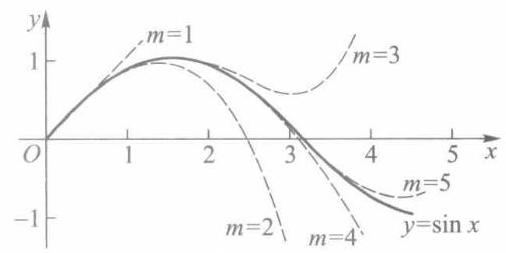
\includegraphics[width=.3\textwidth]{images/P037.jpg}
	\caption{图 $6-6$}
	\label{fig:P037}
\end{figure}

\subsection{习题 6.3}

1. 求下列函数带佩亚诺型余项的麦克劳林公式:

(1) \(f\left( x\right)  = \frac{1}{\sqrt{1 + x}}\) ;

(2) \(f\left( x\right)  = \arctan x\) 到含 \({x}^{5}\) 的项;

(3) \(f\left( x\right)  = \tan x\) 到含 \({x}^{5}\) 的项.

2. 按例 4 的方法求下列极限:

(1) \(\mathop{\lim }\limits_{{x \rightarrow  0}}\frac{{\mathrm{e}}^{x}\sin x - x\left( {1 + x}\right) }{{x}^{3}}\) ;

(2) \(\mathop{\lim }\limits_{{x \rightarrow  \infty }}\left\lbrack  {x - {x}^{2}\ln \left( {1 + \frac{1}{x}}\right) }\right\rbrack\) ;

(3) \(\mathop{\lim }\limits_{{x \rightarrow  0}}\frac{1}{x}\left( {\frac{1}{x} - \cot x}\right)\) .

3. 求下列函数在指定点处带拉格朗日余项的泰勒公式:

(1) \(f\left( x\right)  = {x}^{3} + 4{x}^{2} + 5\) ,在 \(x = 1\) 处；

(2) \(f\left( x\right)  = \frac{1}{1 + x}\) ,在 \(x = 0\) 处.

4. 估计下列近似公式的绝对误差:

(1) \(\sin x \approx  x - \frac{{x}^{3}}{6}\) ,当 \(\left| x\right|  \leq  \frac{1}{2}\) ；

(2) \(\sqrt{1 + x} \approx  1 + \frac{x}{2} - \frac{{x}^{2}}{8},x \in  \left\lbrack  {0,1}\right\rbrack\) .

5. 计算:

(1) 数 \(\mathrm{e}\) 准确到 \({10}^{-9}\) ;

(2) \(\lg {2.7}\) 准确到 \({10}^{-5}\) .

\section{函数的极值与最大 (小) 值}

\subsection{极值判别}

函数的极值不仅在实际问题中占有重要的地位, 而且也是函数性态的一个重要特征.

费马定理 (定理 5.3) 已经告诉我们,若函数 \(f\) 在点 \({x}_{0}\) 可导,且 \({x}_{0}\) 为 \(f\) 的极值点,则 \({f}^{\prime }\left( {x}_{0}\right)  = 0\) . 这就是说,可导函数在点 \({x}_{0}\) 取极值的必要条件是 \({f}^{\prime }\left( {x}_{0}\right)  = 0\) .

下面讨论充分条件.

%定理 6.11
\begin{theorem}{极值的第一充分条件}{the:极值的第一充分条件}
设 \(f\) 在点 \({x}_{0}\) 连续,在某邻域 \({U}^{ \circ  }\left( {{x}_{0};\delta }\right)\) 上可导.

(i) 若当 \(x \in  \left( {{x}_{0} - \delta ,{x}_{0}}\right)\) 时 \({f}^{\prime }\left( x\right)  \leq  0\) ,当 \(x \in  \left( {{x}_{0},{x}_{0} + \delta }\right)\) 时 \({f}^{\prime }\left( x\right)  \geq  0\) ,则 \(f\) 在点 \({x}_{0}\) 取得极小值.

(ii) 若当 \(x \in  \left( {{x}_{0} - \delta ,{x}_{0}}\right)\) 时 \({f}^{\prime }\left( x\right)  \geq  0\) ,当 \(x \in  \left( {{x}_{0},{x}_{0} + \delta }\right)\) 时 \({f}^{\prime }\left( x\right)  \leq  0\) ,则 \(f\) 在点 \({x}_{0}\) 取得极大值.
\end{theorem}


%证
\begin{proof}
下面只证 (ii), (i) 的证明可类似地进行.

由定理的条件及定理 6.3, \(f\) 在 \(\left( {{x}_{0} - \delta ,{x}_{0}}\right)\) 上递增,在 \(\left( {{x}_{0},{x}_{0} + \delta }\right)\) 上递减,又由 \(f\) 在点 \({x}_{0}\) 连续,故对任意 \(x \in  U\left( {{x}_{0};\delta }\right)\) ,恒有
\[
f\left( x\right)  \leq  f\left( {x}_{0}\right) .
\]
即 \(f\) 在点 \({x}_{0}\) 取得极大值.

若 \(f\) 是二阶可导函数,则有如下判别极值定理.
\end{proof}


%定理 6.12
\begin{theorem}{极值的第二充分条件}{the:极值的第二充分条件}
设 \(f\) 在 \({x}_{0}\) 的某邻域 \(U\left( {{x}_{0};\delta }\right)\) 上一阶可导,在 \(x\)  \(= {x}_{0}\) 处二阶可导,且 \({f}^{\prime }\left( {x}_{0}\right)  = 0,{f}^{\prime \prime }\left( {x}_{0}\right)  \neq  0\) .

(i) 若 \({f}^{\prime \prime }\left( {x}_{0}\right)  < 0\) ,则 \(f\) 在 \({x}_{0}\) 取得极大值.

(ii) 若 \({f}^{\prime \prime }\left( {x}_{0}\right)  > 0\) ,则 \(f\) 在 \({x}_{0}\) 取得极小值.
\end{theorem}


%证
\begin{proof}
由条件,可得 \(f\) 在 \({x}_{0}\) 处的二阶泰勒公式
\[
f\left( x\right)  = f\left( {x}_{0}\right)  + {f}^{\prime }\left( {x}_{0}\right) \left( {x - {x}_{0}}\right)  + \frac{1}{2!}{f}^{\prime \prime }\left( {x}_{0}\right) {\left( x - {x}_{0}\right) }^{2} + o\left( {\left( x - {x}_{0}\right) }^{2}\right) .
\]
由于 \({f}^{\prime }\left( {x}_{0}\right)  = 0\) ,因此
\[
f\left( x\right)  - f\left( {x}_{0}\right)  = \left\lbrack  {\frac{{f}^{\prime \prime }\left( {x}_{0}\right) }{2} + o\left( 1\right) }\right\rbrack  {\left( x - {x}_{0}\right) }^{2}. \tag{1}
\]
又因 \({f}^{\prime \prime }\left( {x}_{0}\right)  \neq  0\) ,故存在正数 \({\delta }^{\prime } \leq  \delta\) ,当 \(x \in  U\left( {{x}_{0};{\delta }^{\prime }}\right)\) 时, \(\frac{1}{2}{f}^{\prime \prime }\left( {x}_{0}\right)\) 与 \(\frac{1}{2}{f}^{\prime \prime }\left( {x}_{0}\right)  + o\left( 1\right)\) 同号. 所以,当 \({f}^{\prime \prime }\left( {x}_{0}\right)  < 0\) 时,(1) 式取负值,从而对任意 \(x \in  {U}^{ \circ  }\left( {{x}_{0};{\delta }^{\prime }}\right)\) ,有
\[
f\left( x\right)  - f\left( {x}_{0}\right)  < 0,
\]
即 \(f\) 在 \({x}_{0}\) 取极大值. 同样对 \({f}^{\prime \prime }\left( {x}_{0}\right)  > 0\) ,可得 \(f\) 在点 \({x}_{0}\) 取极小值.
\end{proof}


%例 1
\begin{example}
求 \(f\left( x\right)  = \left( {{2x} - 5}\right) \sqrt[3]{{x}^{2}}\) 的极值点与极值.
\end{example}


%解
\begin{solution}
\(f\left( x\right)  = \left( {{2x} - 5}\right) \sqrt[3]{{x}^{2}} = 2{x}^{\frac{5}{3}} - 5{x}^{\frac{2}{3}}\) 在 \(\left( {-\infty , + \infty }\right)\) 上连续,且当 \(x \neq  0\) 时,有
\[
{f}^{\prime }\left( x\right)  = \frac{10}{3}{x}^{\frac{2}{3}} - \frac{10}{3}{x}^{-\frac{1}{3}} = \frac{10}{3}\frac{x - 1}{\sqrt[3]{x}}.
\]
易见, \(x = 1\) 为 \(f\) 的稳定点, \(x = 0\) 为 \(f\) 的不可导点. 这两点是否是极值点,需作进一步讨论. 现列表如下 (表中\(\nearrow\)表示递增, \(\searrow\) 表示递减):

\begin{center}
    \adjustbox{max width=\textwidth}{
        \begin{tabular}{|c|c|c|c|c|c|}
            \hline
            \(x\) & \(\left( {-\infty ,0}\right)\) & 0 & \((0,1)\) & 1 & \(\left( {1, + \infty }\right)\) \\
            \cline{1-6}
            \({y}^{\prime }\) & \(+\) & 不存在 & \(-\) & 0 & \(+\) \\
            \cline{1-6}
            \(y\) & \(\nearrow\) & 0 & \(\searrow\) & -3 & \(\nearrow\) \\
            \cline{1-6}
            \hline
        \end{tabular}
    }
\end{center}

由上表可见: 点 \(x = 0\) 为 \(f\) 的极大值点,极大值 \(f\left( 0\right)\)  \(= 0;x = 1\) 为 \(f\) 的极小值点,极小值 \(f\left( 1\right)  =  - 3\) (图 6-7).
\end{solution}


\begin{figure}
	\centering
	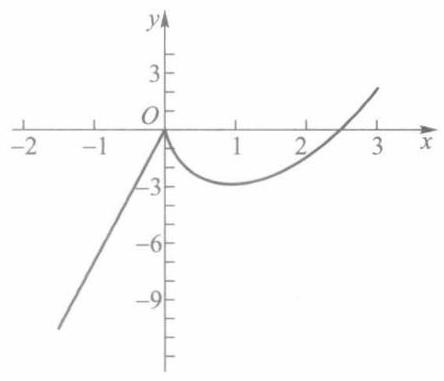
\includegraphics[width=.3\textwidth]{images/P038.jpg}
	\caption{图 $6-7$}
	\label{fig:P038}
\end{figure}

%例 2
\begin{example}
求 \(f\left( x\right)  = {x}^{2} + \frac{432}{x}\) 的极值点与极值.
\end{example}


%解
\begin{solution}
当 \(x \neq  0\) 时,
\[
{f}^{\prime }\left( x\right)  = {2x} - \frac{432}{{x}^{2}} = \frac{2{x}^{3} - {432}}{{x}^{2}}.
\]
令 \({f}^{\prime }\left( x\right)  = 0\) ,求得稳定点 \(x = 6\) . 又因
\[
{f}^{\prime \prime }\left( 6\right)  = {\left( 2 + \frac{864}{{x}^{3}}\right) }_{x = 6} = 6 > 0,
\]
依定理 \({6.12},x = 6\) 为 \(f\) 的极小值点,极小值 \(f\left( 6\right)  = {108}\) .
\end{solution}


对于应用二阶导数无法判别的问题, 可借助更高阶的导数来判别.

%定理 6.13
\begin{theorem}{极值的第三充分条件}{the:极值的第三充分条件}
设 \(f\) 在 \({x}_{0}\) 的某邻域上存在直到 \(n - 1\) 阶导函数,在 \({x}_{0}\) 处 \(n\) 阶可导,且 \({f}^{\left( k\right) }\left( {x}_{0}\right)  = 0\left( {k = 1,2,\cdots ,n - 1}\right) ,{f}^{\left( n\right) }\left( {x}_{0}\right)  \neq  0\) ,则

(i) 当 \(n\) 为偶数时, \(f\) 在 \({x}_{0}\) 取得极值,且当 \({f}^{\left( n\right) }\left( {x}_{0}\right)  < 0\) 时取极大值, \({f}^{\left( n\right) }\left( {x}_{0}\right)  > 0\) 时取极小值.

(ii) 当 \(n\) 为奇数时, \(f\) 在 \({x}_{0}\) 处不取极值.
\end{theorem}

该定理的证明类似于定理 6.12 , 我们将它留给读者.

%例 3
\begin{example}
试求函数 \({x}^{4}{\left( x - 1\right) }^{3}\) 的极值.
\end{example}


%解
\begin{solution}
由于 \({f}^{\prime }\left( x\right)  = {x}^{3}{\left( x - 1\right) }^{2}\left( {{7x} - 4}\right)\) ,因此 \(x = 0,1,\frac{4}{7}\) 是函数的三个稳定点. \(f\) 的二阶导数为
\[
{f}^{\prime \prime }\left( x\right)  = 6{x}^{2}\left( {x - 1}\right) \left( {7{x}^{2} - {8x} + 2}\right) ,
\]
由此得, \({f}^{\prime \prime }\left( 0\right)  = {f}^{\prime \prime }\left( 1\right)  = 0\) 及 \({f}^{\prime \prime }\left( \frac{4}{7}\right)  > 0\) . 所以 \(f\left( x\right)\) 在 \(x = \frac{4}{7}\) 时取得极小值. 求三阶导数
\[
{f}^{\prime \prime \prime }\left( x\right)  = {6x}\left( {{35}{x}^{3} - {60}{x}^{2} + {30x} - 4}\right) ,
\]
有 \({f}^{\prime \prime \prime }\left( 0\right)  = 0,{f}^{\prime \prime \prime }\left( 1\right)  > 0\) . 由于 \(n = 3\) 为奇数,由定理 6.13 知 \(f\) 在 \(x = 1\) 不取极值. 再求 \(f\) 的四阶导数
\[
{f}^{\left( 4\right) }\left( x\right)  = {24}\left( {{35}{x}^{3} - {45}{x}^{2} + {15x} - 1}\right) ,
\]
有 \({f}^{\left( 4\right) }\left( 0\right)  < 0\) . 因为 \(n = 4\) 为偶数,故 \(f\) 在 \(x = 0\) 取得极大值.

综上所述, \(f\left( 0\right)  = 0\) 为极大值,
\[
f\left( \frac{4}{7}\right)  =  - {\left( \frac{4}{7}\right) }^{4}{\left( \frac{3}{7}\right) }^{3} =  - \frac{6912}{823543}
\]
为极小值.
\end{solution}


%注
\begin{remark}
定理 6.13 仍是判定极值的充分条件. 读者可考察函数 (图 6-8)
\[
f\left( x\right)  = \left\{  \begin{array}{ll} {\mathrm{e}}^{-\frac{1}{{x}^{2}}}, & x \neq  0, \\  0, & x = 0. \end{array}\right.
\]
很显然,它在 \(x = 0\) 处取极小值 0 . 但因 \({f}^{\left( k\right) }\left( 0\right)  =\)  \(0,k = 1,2,\cdots\) . 所以无法用定理 6.13 对它作出判别.

\begin{figure}
    \centering
    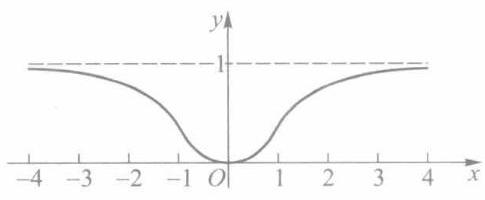
\includegraphics[width=.3\textwidth]{images/P039.jpg}
    \caption{图 $6-8$}
    \label{fig:P039}
\end{figure}
\end{remark}

\subsection{最大值与最小值}

根据闭区间上连续函数的基本性质,若函数 \(f\) 在闭区间 \(\left\lbrack  {a,b}\right\rbrack\) 上连续,则 \(f\) 在 \(\left\lbrack  {a,b}\right\rbrack\) 上一定有最大、最小值. 这就为我们求连续函数的最大、最小值提供了理论保证. 本段将讨论怎样求出这个最大 (小) 值.

若函数 \(f\) 的最大 (小) 值点 \({x}_{0}\) 在开区间(a, b)上,则 \({x}_{0}\) 必定是 \(f\) 的极大 (小) 值点. 又若 \(f\) 在 \({x}_{0}\) 可导,则 \({x}_{0}\) 还是一个稳定点. 所以我们只要比较 \(f\) 在区间内部所有稳定点、 不可导点和区间端点上的函数值,就能从中找到 \(f\) 在 \(\left\lbrack  {a,b}\right\rbrack\) 上的最大值与最小值. 下面举例说明这个求解过程.

%例 4
\begin{example}
求函数 \(f\left( x\right)  = \left| {2{x}^{3} - 9{x}^{2} + {12x}}\right|\) 在闭区间 \(\left\lbrack  {-\frac{1}{4},\frac{5}{2}}\right\rbrack\) 上的最大值与最小值.
\end{example}


%解
\begin{solution}
函数 \(f\) 在闭区间 \(\left\lbrack  {-\frac{1}{4},\frac{5}{2}}\right\rbrack\) 上连续,故必存在最大、最小值. 由于
\[
f\left( x\right)  = \left| {2{x}^{3} - 9{x}^{2} + {12x}}\right|
\]
\[
= \left| {x\left( {2{x}^{2} - {9x} + {12}}\right) }\right|
\]
\[
= \left\{  \begin{array}{ll}  - x\left( {2{x}^{2} - {9x} + {12}}\right) , &  - \frac{1}{4} \leq  x \leq  0, \\  x\left( {2{x}^{2} - {9x} + {12}}\right) , & 0 < x \leq  \frac{5}{2}, \end{array}\right.
\]
因此
\[
{f}^{\prime }\left( x\right)  = \left\{  \begin{array}{l}  - 6{x}^{2} + {18x} - {12} \\  6{x}^{2} - {18x} + {12} \end{array}\right.
\]
\[
= \left\{  \begin{array}{ll}  - 6\left( {x - 1}\right) \left( {x - 2}\right) , &  - \frac{1}{4} \leq  x < 0, \\  6\left( {x - 1}\right) \left( {x - 2}\right) , & 0 < x \leq  \frac{5}{2}. \end{array}\right.
\]
又因 \({f}^{\prime }\left( {0 - 0}\right)  =  - {12},{f}^{\prime }\left( {0 + 0}\right)  = {12}\) ,所以由导数极限定理可知函数在 \(x = 0\) 处不可导. 求出函数 \(f\) 在 \(\left\lbrack  {-\frac{1}{4},\frac{5}{2}}\right\rbrack\) 内部的稳定点 \(x = 1,2\) ,不可导点 \(x = 0\) ,以及端点 \(x =  - \frac{1}{4},\frac{5}{2}\) 的函数值
\[
f\left( 1\right)  = 5,f\left( 2\right)  = 4,f\left( 0\right)  = 0,f\left( {-\frac{1}{4}}\right)  = \frac{115}{32},f\left( \frac{5}{2}\right)  = 5.
\]
所以函数 \(f\) 在 \(x = 0\) 处取最小值 0,在 \(x = 1\) 和 \(x = \frac{5}{2}\) 处取得最大值 5 (图 6-9).
\end{solution}

\begin{figure}
    \centering
    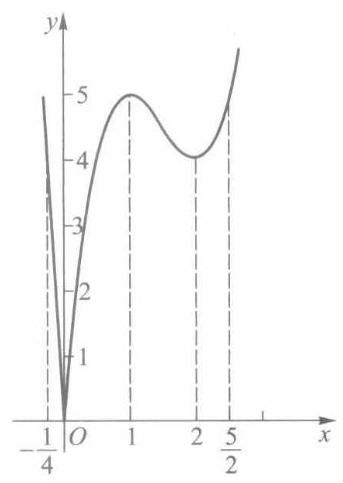
\includegraphics[width=.3\textwidth]{images/P040.jpg}
    \caption{图 $6-9$}
    \label{fig:P040}
\end{figure}

在生产实践和科学实验中, 我们常会遇到求函数的最大值或最小值问题.


%例 5
\begin{example}
一艘轮船在航行中的燃料费和它的速度的立方成正比. 已知当速度为 \({10}\mathrm{\;{km}}/\mathrm{h}\) ,燃料费为每小时 6 元,而其他与速度无关的费用为每小时 96 元. 问轮船的速度为多少时,每航行 \(1\mathrm{\;{km}}\) 所消耗的费用最小?
\end{example}


%解
\begin{solution}
设船速为 \(x\mathrm{\;{km}}/\mathrm{h}\) ,据题意每航行 \(1\mathrm{\;{km}}\) 的耗费为
\[
y = \frac{1}{x}\left( {k{x}^{3} + {96}}\right) .
\]
由已知,当 \(x = {10}\) 时, \(k \cdot  {10}^{3} = 6\) ,故得比例系数 \(k = {0.006}\) . 所以有
\[
y = \frac{1}{x}\left( {{0.006}{x}^{3} + {96}}\right) ,x \in  \left( {0, + \infty }\right) .
\]
令
\[
{y}^{\prime } = \frac{0.012}{{x}^{2}}\left( {{x}^{3} - {8000}}\right)  = 0,
\]
求得稳定点 \(x = {20}\) . 由极值第一充分条件检验得 \(x = {20}\) 是极小值点. 由于在 \(\left( {0, + \infty }\right)\) 上该函数处处可导,且只有唯一的极值点,当它为极小值点时必为最小值点. 所以求得当船速为 \({20}\mathrm{\;{km}}/\mathrm{h}\) 时,每航行 \(1\mathrm{\;{km}}\) 的耗费为最少,其值为 \({y}_{\text{ min }} = {0.006} \times  {20}^{2} + \frac{96}{20}\) =7.2 (元).
\end{solution}


%例 6
\begin{example}
如图 6-10 所示, 剪去正方形四角同样大小的正方形后制成一个无盖盒子, 问剪去小方块的边长为何值时, 可使盒子的容积最大.

\begin{figure}
    \centering
    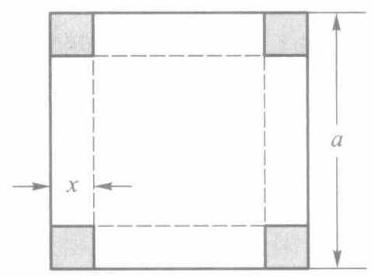
\includegraphics[width=.3\textwidth]{images/P041.jpg}
    \caption{图 $6-10$}
    \label{fig:P041}
\end{figure}
\end{example}


%解
\begin{solution}
设每个小方块边长为 \(x\) ,则盒子的容积为
\[
V\left( x\right)  = x{\left( a - 2x\right) }^{2},x \in  \left\lbrack  {0,\frac{a}{2}}\right\rbrack  .
\]
令
\[
{V}^{\prime }\left( x\right)  = {12}\left( {x - \frac{a}{6}}\right) \left( {x - \frac{a}{2}}\right)  = 0,
\]
在 \(\left( {0,\frac{a}{2}}\right)\) 内解得稳定点 \(x = \frac{a}{6}\) ,并由 \({V}^{\prime \prime }\left( \frac{a}{6}\right)  =  - {4a} < 0\) 知 \(V\left( \frac{a}{6}\right)  = \frac{2{a}^{3}}{27}\) 为极大值. 由于 \(V\left( x\right)\) 在 \(\left( {0,\frac{a}{2}}\right)\) 上只有唯一一个极值点,且为极大值点,因此该极大值就是所求的最大值. 即正方形四个角各剪去一块边长为 \(\frac{a}{6}\) 的小正方形后,能做成容积最大的盒子.
\end{solution}


\subsection{习题 6.4}

1. 求下列函数的极值:

(1) \(f\left( x\right)  = 2{x}^{3} - {x}^{4}\) ;

(2) \(f\left( x\right)  = \frac{2x}{1 + {x}^{2}}\) ;

(3) \(f\left( x\right)  = \frac{{\left( \ln x\right) }^{2}}{x}\) ;

(4) \(f\left( x\right)  = \arctan x - \frac{1}{2}\ln \left( {1 + {x}^{2}}\right)\) .

2. 设
\[
f\left( x\right)  = \left\{  \begin{array}{ll} {x}^{4}{\sin }^{2}\frac{1}{x}, & x \neq  0, \\  0, & x = 0. \end{array}\right.
\]

(1)证明: \(x = 0\) 是极小值点;

(2)说明 \(f\) 在极小值点 \(x = 0\) 是否满足极值的第一充分条件或第二充分条件.

3. 证明:若函数 \(f\) 在点 \({x}_{0}\) 有 \({f}^{\prime }{}_{ + }\left( {x}_{0}\right)  < 0\left( { > 0}\right)\) , \({f}^{\prime }{}_{ - }\left( {x}_{0}\right)  > 0\left( { < 0}\right)\) ,则 \({x}_{0}\) 为 \(f\) 的极大 \(\left( {1\text{ 小 }}\right)\) 值点.

4. 求下列函数在给定区间上的最大、最小值:

(1) \(y = {x}^{5} - 5{x}^{4} + 5{x}^{3} + 1,\left\lbrack  {-1,2}\right\rbrack\) ;

(2) \(y = 2\tan x - {\tan }^{2}x,\left\lbrack  {0,\frac{\pi }{2}}\right)\) ;

(3) \(y = \sqrt{x}\ln x,\left( {0, + \infty }\right)\) .

5. 设 \(f\left( x\right)\) 在区间 \(I\) 上连续,并且在 \(I\) 上仅有唯一的极值点 \({x}_{0}\) . 证明: 若 \({x}_{0}\) 是 \(f\) 的极大 ( 小 ) 值点, 则 \({x}_{0}\) 必是 \(f\left( x\right)\) 在 \(I\) 上的最大 (小) 值点.

6. 把长为 \(l\) 的线段截为两段,问怎样截能使以这两段线为边所组成的矩形的面积最大?

7. 有一个无盖的圆柱形容器,当给定体积为 \(V\) 时,要使容器的表面积为最小,问底的半径与容器高的比例应该怎样?

8. 设用某仪器进行测量时,读得 \(n\) 次实验数据为 \({a}_{1}{a}_{2},\cdots ,{a}_{n}\) . 问以怎样的数值 \(x\) 表达所要测量的真值,才能使它与这 \(n\) 个数之差的平方和为最小?

9. 求一正数 \(a\) ,使它与其倒数之和最小.

10. 求下列函数的极值:


(1) \(f\left( x\right)  = \left| {x\left( {{x}^{2} - 1}\right) }\right|\) ;

(2) \(f\left( x\right)  = \frac{x\left( {{x}^{2} + 1}\right) }{{x}^{4} - {x}^{2} + 1}\) ;

(3) \(f\left( x\right)  = {\left( x - 1\right) }^{2}{\left( x + 1\right) }^{3}\) .

11. 设 \(f\left( x\right)  = a\ln x + b{x}^{2} + x\) 在 \({x}_{1} = 1,{x}_{2} = 2\) 处都取得极值,试求 \(a\) 与 \(b\) ; 并问这时 \(f\) 在 \({x}_{1}\) 与 \({x}_{2}\) 是取得极大值还是极小值?

12. 在抛物线 \({y}^{2} = {2px}\) 上哪一点的法线被抛物线所截之线段为最短?

13. 要把货物从运河边上 \(A\) 城运往与运河相距为 \({BC} = a\mathrm{\;{km}}\) 的 \(B\) 城 (见图 6-11),轮船运费的单价是 \(\alpha\) 元 \(/\mathrm{{km}}\) ,火车运费的单价是 \(\beta\) 元 \(/\mathrm{{km}}\left( {\beta  > \alpha }\right)\) ,试求运河边上的一点 \(M\) ,修建铁路 \({MB}\) ,使得 \(A \rightarrow  M \rightarrow  B\) 的总运费最省.

\begin{figure}
    \centering
    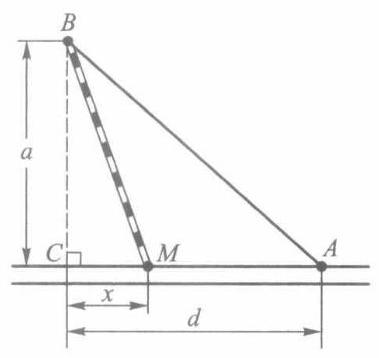
\includegraphics[width=.3\textwidth]{images/P042.jpg}
    \caption{图 $6-11$}
    \label{fig:P042}
\end{figure}

\section{函数的凸性与拐点}

读者已经熟悉函数 \(f\left( x\right)  = {x}^{2}\) 和 \(f\left( x\right)  = \sqrt{x}\) 的图像. 它们不同的特点是: 曲线 \(y = {x}^{2}\) 上任意两点间的弧段总在这两点连线的下方; 而曲线 \(y = \sqrt{x}\) 则相反,任意两点间的弧段总在这两点连线的上方. 我们把具有前一种特性的曲线称为凸的, 相应的函数称为凸函数; 后一种曲线称为凹的, 相应的函数称为凹函数.

%定义  1
\begin{definition}{凸函数和凹函数}{def:凸函数和凹函数}
设 \(f\) 为定义在区间 \(I\) 上的函数,若对 \(I\) 上的任意两点 \({x}_{1},{x}_{2}\) 和任意实数 \(\lambda\)  \(\in  \left( {0,1}\right)\) ,总有
\[
f\left( {\lambda {x}_{1} + \left( {1 - \lambda }\right) {x}_{2}}\right)  \leq  {\lambda f}\left( {x}_{1}\right)  + \left( {1 - \lambda }\right) f\left( {x}_{2}\right) , \tag{1}
\]
则称 \(f\) 为 \(I\) 上的凸函数. 反之,如果总有
\[
f\left( {\lambda {x}_{1} + \left( {1 - \lambda }\right) {x}_{2}}\right)  \geq  {\lambda f}\left( {x}_{1}\right)  + \left( {1 - \lambda }\right) f\left( {x}_{2}\right) , \tag{2}
\]
则称 \(f\) 为 \(I\) 上的凹函数.

如果 (1)、(2) 中的不等式改为严格不等式, 则相应的函数称为严格凸函数和严格凹函数.
\end{definition}


图 6-12 中的 (a) 和 (b) 分别是凸函数和凹函数的几何形状,其中 \(x = \lambda {x}_{1} + (1 -\)  \(\lambda ){x}_{2},A = f\left( {x}_{1}\right) ,B = f\left( {x}_{2}\right) ,C = {\lambda A} + \left( {1 - \lambda }\right) B\) .

\begin{figure}
    \centering
    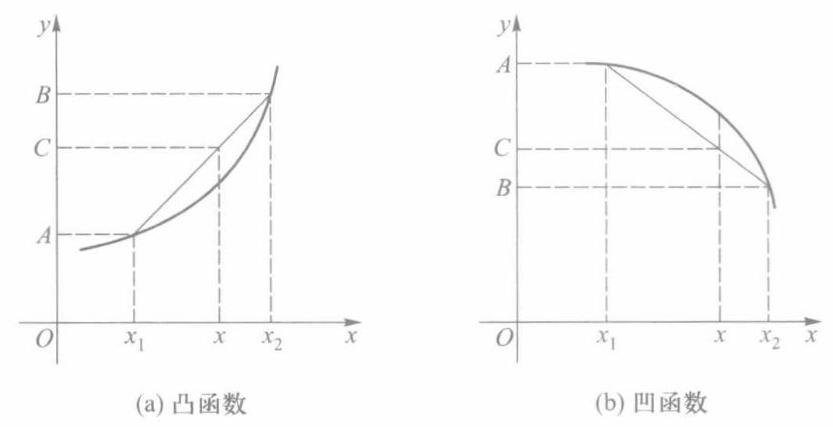
\includegraphics[width=.3\textwidth]{images/P043.jpg}
    \caption{图 $6-12$}
    \label{fig:P043}
\end{figure}

容易证明: 若 \(- f\) 为区间 \(I\) 上的凸函数,则 \(f\) 为区间 \(I\) 上的凹函数. 因此,今后只需讨论凸函数的性质即可.

%引理
\begin{lemma}{引理}{pro:引理}
\(f\) 为 \(I\) 上的凸函数的充要条件是: 对于 \(I\) 上的任意三点 \({x}_{1} < {x}_{2} < {x}_{3}\) ,总有
\[
\frac{f\left( {x}_{2}\right)  - f\left( {x}_{1}\right) }{{x}_{2} - {x}_{1}} \leq  \frac{f\left( {x}_{3}\right)  - f\left( {x}_{2}\right) }{{x}_{3} - {x}_{2}}. \tag{3}
\]
\end{lemma}

%证
\begin{proof}
必要性 记 \(\lambda  = \frac{{x}_{3} - {x}_{2}}{{x}_{3} - {x}_{1}}\) ,则 \({x}_{2} = \lambda {x}_{1} + \left( {1 - \lambda }\right) {x}_{3}\) . 由 \(f\) 的凸性知道
\[
f\left( {x}_{2}\right)  = f\left( {\lambda {x}_{1} + \left( {1 - \lambda }\right) {x}_{3}}\right)  \leq  {\lambda f}\left( {x}_{1}\right)  + \left( {1 - \lambda }\right) f\left( {x}_{3}\right)
\]
\[
= \frac{{x}_{3} - {x}_{2}}{{x}_{3} - {x}_{1}}f\left( {x}_{1}\right)  + \frac{{x}_{2} - {x}_{1}}{{x}_{3} - {x}_{1}}f\left( {x}_{3}\right) ,
\]

从而有
\[
\left( {{x}_{3} - {x}_{1}}\right) f\left( {x}_{2}\right)  \leq  \left( {{x}_{3} - {x}_{2}}\right) f\left( {x}_{1}\right)  + \left( {{x}_{2} - {x}_{1}}\right) f\left( {x}_{3}\right) ,
\]
\[
\left( {{x}_{3} - {x}_{2}}\right) f\left( {x}_{2}\right)  + \left( {{x}_{2} - {x}_{1}}\right) f\left( {x}_{2}\right)  \leq  \left( {{x}_{3} - {x}_{2}}\right) f\left( {x}_{1}\right)  + \left( {{x}_{2} - {x}_{1}}\right) f\left( {x}_{3}\right) ,
\]
整理后即得 (3) 式.

充分性 如图 6-13 所示,在 \(I\) 上任取两点 \({x}_{1},{x}_{3}\left( {{x}_{1} < {x}_{3}}\right)\) ,在 \(\left\lbrack  {{x}_{1},{x}_{3}}\right\rbrack\) 上任取一点 \({x}_{2} = \lambda {x}_{1} + \left( {1 - \lambda }\right) {x}_{3},\lambda  \in  \left( {0,1}\right)\) ,即 \(\lambda  = \frac{{x}_{3} - {x}_{2}}{{x}_{3} - {x}_{1}}\) . 由必要性的推导逆过程,可推得
\[
f\left( {\lambda {x}_{1} + \left( {1 - \lambda }\right) {x}_{3}}\right)  \leq  {\lambda f}\left( {x}_{1}\right)  + \left( {1 - \lambda }\right) f\left( {x}_{3}\right) ,
\]
故 \(f\) 为 \(I\) 上的凸函数.


\begin{figure}
    \centering
    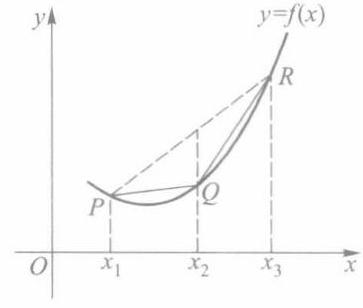
\includegraphics[width=.3\textwidth]{images/P044.jpg}
    \caption{图 $6-13$}
    \label{fig:P044}
\end{figure}
\end{proof}


同理可证, \(f\) 为 \(I\) 上的凸函数的充要条件是: 对于 \(I\) 上任意三点 \({x}_{1} < {x}_{2} < {x}_{3}\) ,有
\[
\frac{f\left( {x}_{2}\right)  - f\left( {x}_{1}\right) }{{x}_{2} - {x}_{1}} \leq  \frac{f\left( {x}_{3}\right)  - f\left( {x}_{1}\right) }{{x}_{3} - {x}_{1}}
\]
\[
\leq  \frac{f\left( {x}_{3}\right)  - f\left( {x}_{2}\right) }{{x}_{3} - {x}_{2}}. \tag{4}
\]

%注
\begin{remark}
如果 \(f\left( x\right)\) 为 \(I\) 上的严格凸函数,则不等式 (3) 和 (4) 中的“ \(\leq\) ”可改为“ \(<\) ”.
\end{remark}


%定理 6.14
\begin{theorem}{可导等价}{the:可导等价}
设 \(f\) 为区间 \(I\) 上的可导函数,则下述论断互相等价:

\({1}^{ \circ  }f\) 为 \(I\) 上凸函数;

\({2}^{ \circ  }{f}^{\prime }\) 为 \(I\) 上的增函数;

\({3}^{ \circ  }\) 对 \(I\) 上的任意两点 \({x}_{1},{x}_{2}\) ,有
\[
f\left( {x}_{2}\right)  \geq  f\left( {x}_{1}\right)  + {f}^{\prime }\left( {x}_{1}\right) \left( {{x}_{2} - {x}_{1}}\right) . \tag{5}
\]
\end{theorem}

%证
\begin{proof}
\(\left( {{1}^{ \circ  } \rightarrow  {2}^{ \circ  }}\right)\) 任取 \(I\) 上两点 \({x}_{1},{x}_{2}\left( {{x}_{1} < {x}_{2}}\right)\) 及充分小的正数 \(h\) . 由于 \({x}_{1} - h < {x}_{1} < {x}_{2} < {x}_{2} + h\) ,根据 \(f\) 的凸性及引理有
\[
\frac{f\left( {x}_{1}\right)  - f\left( {{x}_{1} - h}\right) }{h} \leq  \frac{f\left( {x}_{2}\right)  - f\left( {x}_{1}\right) }{{x}_{2} - {x}_{1}} \leq  \frac{f\left( {{x}_{2} + h}\right)  - f\left( {x}_{2}\right) }{h}.
\]
由 \(f\) 是可导函数,令 \(h \rightarrow  {0}^{ + }\) 时可得
\[
{f}^{\prime }\left( {x}_{1}\right)  \leq  \frac{f\left( {x}_{2}\right)  - f\left( {x}_{1}\right) }{{x}_{2} - {x}_{1}} \leq  {f}^{\prime }\left( {x}_{2}\right) ,
\]
所以 \({f}^{\prime }\) 为 \(I\) 上的递增函数.

\(\left( {{2}^{ \circ  } \rightarrow  {3}^{ \circ  }}\right)\) 在以 \({x}_{1},{x}_{2}\left( {{x}_{1} < {x}_{2}}\right)\) 为端点的区间上,应用拉格朗日中值定理和 \({f}^{\prime }\) 递增条件, 有
\[
f\left( {x}_{2}\right)  - f\left( {x}_{1}\right)  = {f}^{\prime }\left( \xi \right) \left( {{x}_{2} - {x}_{1}}\right)  \geq  {f}^{\prime }\left( {x}_{1}\right) \left( {{x}_{2} - {x}_{1}}\right) .
\]
移项后即得 (5) 式成立,且当 \({x}_{1} > {x}_{2}\) 时仍可得到相同结论.

\(\left( {{3}^{ \circ  } \rightarrow  {1}^{ \circ  }}\right)\) 设 \({x}_{1},{x}_{2}\) 为 \(I\) 上任意两点, \({x}_{3} = \lambda {x}_{1} + \left( {1 - \lambda }\right) {x}_{2},0 < \lambda  < 1\) . 由 \({3}^{ \circ  }\) ,并利用 \({x}_{1} -\)  \({x}_{3} = \left( {1 - \lambda }\right) \left( {{x}_{1} - {x}_{2}}\right)\) 与 \({x}_{2} - {x}_{3} = \lambda \left( {{x}_{2} - {x}_{1}}\right)\) ,有
\[
f\left( {x}_{1}\right)  \geq  f\left( {x}_{3}\right)  + {f}^{\prime }\left( {x}_{3}\right) \left( {{x}_{1} - {x}_{3}}\right)  = f\left( {x}_{3}\right)  + \left( {1 - \lambda }\right) {f}^{\prime }\left( {x}_{3}\right) \left( {{x}_{1} - {x}_{2}}\right) ,
\]
\[
f\left( {x}_{2}\right)  \geq  f\left( {x}_{3}\right)  + {f}^{\prime }\left( {x}_{3}\right) \left( {{x}_{2} - {x}_{3}}\right)  = f\left( {x}_{3}\right)  + \lambda {f}^{\prime }\left( {x}_{3}\right) \left( {{x}_{2} - {x}_{1}}\right) .
\]
分别用 \(\lambda\) 和 \(1 - \lambda\) 乘上列两式并相加,便得
\[
{\lambda f}\left( {x}_{1}\right)  + \left( {1 - \lambda }\right) f\left( {x}_{2}\right)  \geq  f\left( {x}_{3}\right)  = f\left( {\lambda {x}_{1} + \left( {1 - \lambda }\right) {x}_{2}}\right) .
\]
从而 \(f\) 为 \(I\) 上的凸函数.
\end{proof}


注意 论断 \({3}^{ \circ  }\) 的几何意义是: 曲线 \(y = f\left( x\right)\) 总是在它的任一切线的上方 (图 6-14). 这是可导凸函数的几何特征.

对于凹函数, 同样有类似于定理 6.14 的结论.

\begin{figure}
	\centering
	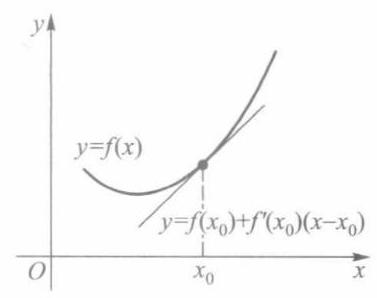
\includegraphics[width=.3\textwidth]{images/P045.jpg}
	\caption{图 $6-14$}
	\label{fig:P045}
\end{figure}

%定理 6.15
\begin{theorem}{二阶可导函数}{the:二阶可导函数}
设 \(f\) 为区间 \(I\) 上的二阶可导函数,则在 \(I\) 上 \(f\) 为凸 (凹) 函数的充要条件是
\[
{f}^{\prime \prime }\left( x\right)  \geq  0\left( {{f}^{\prime \prime }\left( x\right)  \leq  0}\right) ,x \in  I.
\]
\end{theorem}

这个定理的结论可由定理 6.3 和定理 6.14 推出.

%例 1
\begin{example}
讨论函数 \(f\left( x\right)  = \arctan x\) 的凸 (凹) 性区间.
\end{example}


%解
\begin{solution}
由于 \({f}^{\prime \prime }\left( x\right)  = \frac{-{2x}}{{\left( 1 + {x}^{2}\right) }^{2}}\) ,因而当 \(x \leq  0\) 时, \({f}^{\prime \prime }\left( x\right)  \geq\)  \(0;x \geq  0\) 时, \({f}^{\prime \prime }\left( x\right)  \leq  0\) . 从而在 \(( - \infty ,0\rbrack\) 上 \(f\) 为凸函数,在 \(\lbrack 0, + \infty )\) 上 \(f\) 为凹函数.
\end{solution}


%例 2
\begin{example}
若函数 \(f\) 为定义在开区间(a, b)上的可导的凸 (凹) 函数,则 \({x}_{0} \in  \left( {a,b}\right)\) 为 \(f\) 的极小 (大) 值点的充要条件是 \({x}_{0}\) 为 \(f\) 的稳定点,即 \({f}^{\prime }\left( {x}_{0}\right)  = 0\) .
\end{example}

%证
\begin{proof}
下面只证明 \(f\) 为凸函数的情形.

必要性已由费马定理给出, 现在证明充分性.

由定理 6.14,任取(a, b)上的一点 \(x\left( { \neq  {x}_{0}}\right)\) ,它与 \({x}_{0}\) 一起有
\[
f\left( x\right)  \geq  f\left( {x}_{0}\right)  + {f}^{\prime }\left( {x}_{0}\right) \left( {x - {x}_{0}}\right) .
\]
因为 \({f}^{\prime }\left( {x}_{0}\right)  = 0\) ,故对任何 \(x \in  \left( {a,b}\right)\) ,总有
\[
f\left( x\right)  \geq  f\left( {x}_{0}\right) ,
\]
即 \({x}_{0}\) 为 \(f\) 在(a, b)上的极小值点 (而且为最小值点).
\end{proof}


%例 3
\begin{example}
设 \(f\left( x\right)\) 为区间(a, b)上的凸函数,不恒为常数. 证明: \(f\left( x\right)\) 不取最大值.
\end{example}


%证
\begin{proof}
若不然,可设 \(f\left( {x}_{0}\right)\) 是最大值. 由凸函数的定义,对于任意 \({x}_{1},{x}_{2} \in  \left( {a,b}\right) ,{x}_{1} <\)  \({x}_{0} < {x}_{2}\) ,有
\[
f\left( {x}_{0}\right)  \leq  \frac{{x}_{2} - {x}_{0}}{{x}_{2} - {x}_{1}}f\left( {x}_{1}\right)  + \frac{{x}_{0} - {x}_{1}}{{x}_{2} - {x}_{1}}f\left( {x}_{2}\right)
\]
\[
\leq  \left( {\frac{{x}_{2} - {x}_{0}}{{x}_{2} - {x}_{1}} + \frac{{x}_{0} - {x}_{1}}{{x}_{2} - {x}_{1}}}\right) f\left( {x}_{0}\right)  = f\left( {x}_{0}\right) ,
\]
从而得到 \(f\left( {x}_{0}\right)  = f\left( {x}_{1}\right)  = f\left( {x}_{2}\right)\) ,即 \(f\left( x\right)\) 是常量函数,矛盾.
\end{proof}


%注
\begin{remark}
若 \(f\left( x\right)\) 是区间 \(\left\lbrack  {a,b}\right\rbrack\) 上的凸的连续函数,那么
\[
f\left( x\right)  \leq  \max \{ f\left( a\right) ,f\left( b\right) \} .
\]
\end{remark}

%例 4
\begin{example}
求证 \(1 + {x}^{2} \leq  {2}^{x} \leq  1 + x,x \in  \left\lbrack  {0,1}\right\rbrack\) .
\end{example}


%证
\begin{proof}
设 \(f\left( x\right)  = 1 + {x}^{2} - {2}^{x},g\left( x\right)  = {2}^{x} - 1 - x\) ,那么
\[
{f}^{\prime \prime }\left( x\right)  = 2 - {2}^{x}{\left( \ln 2\right) }^{2} \geq  0,\;{g}^{\prime \prime }\left( x\right)  = {2}^{x}{\left( \ln 2\right) }^{2} > 0.
\]
因此 \(f\left( x\right) ,g\left( x\right)\) 均为 \(\left\lbrack  {0,1}\right\rbrack\) 上的凸函数,故由例 3 得
\[
f\left( x\right)  \leq  \max \{ f\left( 0\right) ,f\left( 1\right) \}  = 0,\;g\left( x\right)  \leq  \max \{ g\left( 0\right) ,g\left( 1\right) \}  = 0.
\]
由此推得所需的结果.
\end{proof}


下例是定义 1 的一般情形.

%例 5
\begin{example}
(延森 (Jensen) 不等式) 若 \(f\) 为 \(\left\lbrack  {a,b}\right\rbrack\) 上的凸函数,则对任意 \({x}_{i} \in  \left\lbrack  {a,b}\right\rbrack  ,{\lambda }_{i} > 0\)  \(\left( {i = 1,2,\cdots ,n}\right) ,\mathop{\sum }\limits_{{i = 1}}^{n}{\lambda }_{i} = 1\) ,有
\[
f\left( {\mathop{\sum }\limits_{{i = 1}}^{n}{\lambda }_{i}{x}_{i}}\right)  \leq  \mathop{\sum }\limits_{{i = 1}}^{n}{\lambda }_{i}f\left( {x}_{i}\right) . \tag{6}
\]
\end{example}

%证
\begin{proof}
应用数学归纳法. 当 \(n = 2\) 时,由定义 1,命题显然成立. 设 \(n = k\) 时命题成立. 即对任意 \({x}_{1},{x}_{2},\cdots ,{x}_{k} \in  \left\lbrack  {a,b}\right\rbrack\) 及
\[
{\alpha }_{i} > 0,i = 1,2,\cdots ,k,\mathop{\sum }\limits_{{i = 1}}^{k}{\alpha }_{i} = 1,
\]
都有
\[
f\left( {\mathop{\sum }\limits_{{i = 1}}^{k}{\alpha }_{i}{x}_{i}}\right)  \leq  \mathop{\sum }\limits_{{i = 1}}^{k}{\alpha }_{i}f\left( {x}_{i}\right) .
\]
现设 \({x}_{1},{x}_{2},\cdots ,{x}_{k},{x}_{k + 1} \in  \left\lbrack  {a,b}\right\rbrack\) 及
\[
{\lambda }_{i} > 0\left( {i = 1,2,\cdots ,k + 1}\right) ,\mathop{\sum }\limits_{{i = 1}}^{{k + 1}}{\lambda }_{i} = 1.
\]
令 \({\alpha }_{i} = \frac{{\lambda }_{i}}{1 - {\lambda }_{k + 1}},i = 1,2,\cdots ,k\) ,则 \(\mathop{\sum }\limits_{{i = 1}}^{k}{\alpha }_{i} = 1\) . 由数学归纳法假设可推得
\[
f\left( {{\lambda }_{1}{x}_{1} + {\lambda }_{2}{x}_{2} + \cdots  + {\lambda }_{k}{x}_{k} + {\lambda }_{k + 1}{x}_{k + 1}}\right)
\]
\[
= f\left( {\left( {1 - {\lambda }_{k + 1}}\right) \frac{{\lambda }_{1}{x}_{1} + {\lambda }_{2}{x}_{2} + \cdots  + {\lambda }_{k}{x}_{k}}{1 - {\lambda }_{k + 1}} + {\lambda }_{k + 1}{x}_{k + 1}}\right)
\]
\[
\leq  \left( {1 - {\lambda }_{k + 1}}\right) f\left( {{\alpha }_{1}{x}_{1} + {\alpha }_{2}{x}_{2} + \cdots  + {\alpha }_{k}{x}_{k}}\right)  + {\lambda }_{k + 1}f\left( {x}_{k + 1}\right)
\]
\[
\leq  \left( {1 - {\lambda }_{k + 1}}\right) \left\lbrack  {{\alpha }_{1}f\left( {x}_{1}\right)  + {\alpha }_{2}f\left( {x}_{2}\right)  + \cdots  + {\alpha }_{k}f\left( {x}_{k}\right) }\right\rbrack   + {\lambda }_{k + 1}f\left( {x}_{k + 1}\right)
\]
\[
= \left( {1 - {\lambda }_{k + 1}}\right) \left\lbrack  {\frac{{\lambda }_{1}}{1 - {\lambda }_{k + 1}}f\left( {x}_{1}\right)  + \frac{{\lambda }_{2}}{1 - {\lambda }_{k + 1}}f\left( {x}_{2}\right)  + \cdots  + \frac{{\lambda }_{k}}{1 - {\lambda }_{k + 1}}f\left( {x}_{k}\right) }\right\rbrack   +
\]
\[
{\lambda }_{k + 1}f\left( {x}_{k + 1}\right)  = \mathop{\sum }\limits_{{i = 1}}^{{k + 1}}{\lambda }_{i}f\left( {x}_{i}\right) .
\]
这就证明了对任何正整数 \(n\left( { \geq  2}\right)\) ,凸函数 \(f\) 总有不等式 (6) 成立.
\end{proof}


%注
\begin{remark}
如 \(f\left( x\right)\) 在 \(\left\lbrack  {a,b}\right\rbrack\) 上严格凸,则 (6) 式可为严格不等式,除非 \({x}_{1} = {x}_{2} = \cdots  = {x}_{n}\) .
\end{remark}


%例 6
\begin{example}
证明不等式 \({\left( abc\right) }^{\frac{a + b + c}{3}} \leq  {a}^{a}{b}^{b}{c}^{c}\) ,其中 \(a,b,c\) 均为正数.
\end{example}

%证
\begin{proof}
设 \(f\left( x\right)  = x\ln x,x > 0\) . 由 \(f\left( x\right)\) 的一阶和二阶导数
\[
{f}^{\prime }\left( x\right)  = \ln x + 1,\;{f}^{\prime \prime }\left( x\right)  = \frac{1}{x},
\]
可见, \(f\left( x\right)  = x\ln x\) 在 \(x > 0\) 时为严格凸函数. 依延森不等式有
\[
f\left( \frac{a + b + c}{3}\right)  \leq  \frac{1}{3}\left\lbrack  {f\left( a\right)  + f\left( b\right)  + f\left( c\right) }\right\rbrack  ,
\]
从而
\[
\frac{a + b + c}{3}\ln \frac{a + b + c}{3} \leq  \frac{1}{3}\left( {a\ln a + b\ln b + c\ln c}\right) ,
\]
即
\[
{\left( \frac{a + b + c}{3}\right) }^{a + b + c} \leq  {a}^{a}{b}^{b}{c}^{c}.
\]
又因 \(\sqrt[3]{abc} \leq  \frac{a + b + c}{3}\) ,所以
\[
{\left( abc\right) }^{\frac{a + b + c}{3}} \leq  {a}^{a}{b}^{b}{c}^{c}.
\]
\end{proof}

%例 7
\begin{example}
设 \(A,B,C\) 是三角形的三个内角,证明
\[
\sin A + \sin B + \sin C \leq  \frac{3}{2}\sqrt{3}\text{ . }
\]
\end{example}

%证
\begin{proof}
设 \(f\left( x\right)  = \sin x,x \in  \left\lbrack  {0,\pi }\right\rbrack\) . 由于 \({f}^{\prime \prime }\left( x\right)  =  - \sin x < 0\) ,因而 \(f\left( x\right)\) 是严格凹函数. 由延森不等式,
\[
\sin A + \sin B + \sin C \leq  3\sin \frac{A + B + C}{3} = \frac{3}{2}\sqrt{3}\text{ . }
\]
等号成立当且仅当 \(A = B = C = \frac{\pi }{3}\) .
\end{proof}


%例 8
\begin{example}
设 \(f\) 为开区间 \(I\) 上的凸 (凹) 函数,证明 \(f\) 在 \(I\) 上任一点 \({x}_{0}\) 都存在左、右导数.
\end{example}


%证
\begin{proof}
下面只证凸函数 \(f\) 在点 \({x}_{0}\) 存在右导数,同理可证也存在左导数和 \(f\) 为凹函数的情形.

设 \(0 < {h}_{1} < {h}_{2}\) ,则对 \({x}_{0} < {x}_{0} + {h}_{1} < {x}_{0} + {h}_{2}\) (这里取充分小的 \({h}_{2}\) ,使 \({x}_{0} +\)  \(\left. {{h}_{2} \in  I}\right)\) ,由引理中的 (4) 式有
\[
\frac{f\left( {{x}_{0} + {h}_{1}}\right)  - f\left( {x}_{0}\right) }{{h}_{1}} \leq  \frac{f\left( {{x}_{0} + {h}_{2}}\right)  - f\left( {x}_{0}\right) }{{h}_{2}}.
\]
令 \(F\left( h\right)  = \frac{f\left( {{x}_{0} + h}\right)  - f\left( {x}_{0}\right) }{h}\) ,故由上式可见 \(F\) 为增函数. 任取 \({x}^{\prime } \in  I\) 且 \({x}^{\prime } < {x}_{0}\) ,则对任何 \(h >\) 0,只要 \({x}_{0} + h \in  I\) ,也有
\[
\frac{f\left( {x}_{0}\right)  - f\left( {x}^{\prime }\right) }{{x}_{0} - {x}^{\prime }} \leq  \frac{f\left( {{x}_{0} + h}\right)  - f\left( {x}_{0}\right) }{h} = F\left( h\right) .
\]
由于上式左端是一个定数,因而函数 \(F\left( h\right)\) 在 \(h > 0\) 上有下界. 根据定理 3.10,极限 \(F\left( h\right)\) 存在,即 \({f}^{\prime }{}_{ + }\left( {x}_{0}\right)\) 存在.
\end{proof}


%定义  2
\begin{definition}{拐点}{def:拐点}
设曲线 \(y = f\left( x\right)\) 在点 \(\left( {{x}_{0},f\left( {x}_{0}\right) }\right)\) 处有穿过曲线的切线. 且在切点近旁,曲线在切线的两侧分别是严格凸和严格凹的, 这时称点 \(\left( {{x}_{0},f\left( {x}_{0}\right) }\right)\) 为曲线 \(y = f\left( x\right)\) 的拐点.
\end{definition}


\begin{figure}
	\centering
	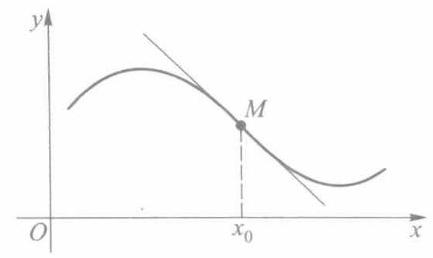
\includegraphics[width=.3\textwidth]{images/P046.jpg}
	\caption{图 $6-15$}
	\label{fig:P046}
\end{figure}

由定义可见, 拐点正是凸和凹曲线的分界点, 如图 6-15 中的点 \(M\) .

例 1 中的点(0,0)为 \(y = \arctan x\) 的拐点. 容易验证: 正弦曲线 \(y = \sin x\) 有拐点 \(\left( {{k\pi },0}\right) ,k\) 为整数.

读者容易证明下述两个有关拐点的定理.

%定理 6.16
\begin{theorem}{二阶可导拐点}{the:二阶可导拐点}
若 \(f\) 在 \({x}_{0}\) 二阶可导,则 \(\left( {{x}_{0},f\left( {x}_{0}\right) }\right)\) 为曲线 \(y = f\left( x\right)\) 的拐点的必要条件是 \({f}^{\prime \prime }\left( {x}_{0}\right)  = 0\) .
\end{theorem}


%定理 6.17
\begin{theorem}{二阶可导拐点2}{the:二阶可导拐点2}
设 \(f\) 在 \({x}_{0}\) 可导,在某邻域 \({U}^{ \circ  }\left( {x}_{0}\right)\) 上二阶可导. 若在 \({U}_{ + }^{ \circ  }\left( {x}_{0}\right)\) 和 \({U}_{ - }^{ \circ  }\left( {x}_{0}\right)\) 上 \({f}^{\prime \prime }\left( x\right)\) 的符号相反,则 \(\left( {{x}_{0},f\left( {x}_{0}\right) }\right)\) 为曲线 \(y = f\left( x\right)\) 的拐点.
\end{theorem}


必须指出: 若 \(\left( {{x}_{0},f\left( {x}_{0}\right) }\right)\) 是曲线 \(y = f\left( x\right)\) 的一个拐点, \(y = f\left( x\right)\) 在 \({x}_{0}\) 的导数不一定存在. 请考察函数 \(y = \sqrt[3]{x}\) 在 \(x = 0\) 的情况.

\subsection{习题 6.5}

1. 确定下列函数的凸性区间与拐点:

(1) \(y = 2{x}^{3} - 3{x}^{2} - {36x} + {25}\) ;

(2) \(y = x + \frac{1}{x}\) ;

(3) \(y = {x}^{2} + \frac{1}{x}\) ;

(4) \(y = \ln \left( {{x}^{2} + 1}\right)\) ;

(5) \(y = \frac{1}{1 + {x}^{2}}\) .

2. 问 \(a\) 和 \(b\) 为何值时,点(1,3)为曲线 \(y = a{x}^{3} + b{x}^{2}\) 的拐点?

3. 证明:

(1)若 \(f\) 为凸函数, \(\lambda\) 为非负实数,则 \({\lambda f}\) 为凸函数；

(2)若 \(f,g\) 均为凸函数,则 \(f + g\) 为凸函数；

(3)若 \(f\) 为区间 \(I\) 上凸函数, \(g\) 为 \(J \supset  f\left( I\right)\) 上凸增函数,则 \(g \circ  f\) 为 \(I\) 上凸函数.

4. 设 \(f\) 为区间 \(I\) 上严格凸函数. 证明: 若 \({x}_{0} \in  I\) 为 \(f\) 的极小值点,则 \({x}_{0}\) 为 \(f\) 在 \(I\) 上唯一的极小值点.

5. 应用凸函数概念证明如下不等式:

(1)对任意实数 \(a,b\) ,有 \({\mathrm{e}}^{\frac{a + b}{2}} \leq  \frac{1}{2}\left( {{\mathrm{e}}^{a} + {\mathrm{e}}^{b}}\right)\) ；

(2)对任何非负实数 \(a,b\) ,有 \(2\arctan \left( \frac{a + b}{2}\right)  \geq  \arctan a + \arctan b\) .

6. 证明: \(\sin {\pi x} \leq  \frac{{\pi }^{2}}{2}x\left( {1 - x}\right)\) ,其中 \(x \in  \left\lbrack  {0,1}\right\rbrack\) .

7. 证明: 若 \(f,g\) 均为区间 \(I\) 上凸函数,则 \(F\left( x\right)  = \max \{ f\left( x\right) ,g\left( x\right) \}\) 也是 \(I\) 上凸函数.

8. 证明: \(\left( 1\right) f\) 为区间 \(I\) 上凸函数的充要条件是对 \(I\) 上任意三点 \({x}_{1} < {x}_{2} < {x}_{3}\) ,恒有
\[
\Delta  = \left| \begin{array}{lll} 1 & {x}_{1} & f\left( {x}_{1}\right) \\  1 & {x}_{2} & f\left( {x}_{2}\right) \\  1 & {x}_{3} & f\left( {x}_{3}\right)  \end{array}\right|  \geq  0;
\]
(2) \(f\) 为严格凸函数的充要条件是 \(\Delta  > 0\) .

9. 应用延森不等式证明:

(1)设 \({a}_{i} > 0\left( {i = 1,2,\cdots ,n}\right)\) ,有
\[
\frac{n}{\frac{1}{{a}_{1}} + \frac{1}{{a}_{2}} + \cdots  + \frac{1}{{a}_{n}}} \leq  \sqrt[n]{{a}_{1}{a}_{2}\cdots {a}_{n}} \leq  \frac{{a}_{1} + {a}_{2} + \cdots  + {a}_{n}}{n};
\]

(2)设 \({a}_{i},{b}_{i} > 0\left( {i = 1,2,\cdots ,n}\right)\) ,有
\[
\mathop{\sum }\limits_{{i = 1}}^{n}{a}_{i}{b}_{i} \leq  {\left( \mathop{\sum }\limits_{{i = 1}}^{n}{a}_{i}^{p}\right) }^{\frac{1}{p}}{\left( \mathop{\sum }\limits_{{i = 1}}^{n}{b}_{i}^{q}\right) }^{\frac{1}{q}},
\]
其中 \(p > 1,q > 1,\frac{1}{p} + \frac{1}{q} = 1\) .

10. 求证:圆内接 \(n\) 边形的面积最大者必为正 \(n\) 边形 \(\left( {n \geq  3}\right)\) .

\section{函数图像的讨论}

在中学里, 我们主要依赖描点作图法画出一些简单函数的图像. 一般来说, 这样得到的图像比较粗糙,无法确切反映函数的性态 (如单调区间、极值点、凸性区间、拐点等).这一节里,我们将综合应用在本章前几节学过的方法,再综合周期性、奇偶性、渐近线等知识, 较完善地作出函数的图像.

作函数图像的一般程序是:

1. 求函数的定义域；

2. 考察函数的奇偶性、周期性;

3. 求函数的某些特殊点,如与两个坐标轴的交点、不连续点、不可导点等；

4. 确定函数的单调区间、极值点、凸性区间以及拐点；

5. 考察渐近线;

6. 综合以上讨论结果画出函数图像.

下面举例说明如何按照上述程序作出函数的图像.

%例
\begin{example}
讨论函数 \(f\left( x\right)  = \sqrt[3]{{x}^{3} - {x}^{2} - x + 1}\) 的性态,并作出其图像.
\end{example}

%解
\begin{solution}
由于
\[
f\left( x\right)  = \sqrt[3]{{x}^{3} - {x}^{2} - x + 1} = \sqrt[3]{{\left( x - 1\right) }^{2}} \cdot  \sqrt[3]{x + 1},
\]
可见此曲线与坐标轴交于 \(\left( {1,0}\right) ,\left( {-1,0}\right) ,\left( {0,1}\right)\) 三点.

求出导数:
\[
{f}^{\prime }\left( x\right)  = \frac{2}{3}\frac{\sqrt[3]{x + 1}}{\sqrt[3]{x - 1}} + \frac{1}{3} \cdot  \frac{\sqrt[3]{{\left( x - 1\right) }^{2}}}{\sqrt[3]{{\left( x + 1\right) }^{2}}} = \frac{x + \frac{1}{3}}{\sqrt[3]{x - 1} \cdot  \sqrt[3]{{\left( x + 1\right) }^{2}}},
\]
由此得到稳定点 \(x =  - \frac{1}{3}\) ,不可导点 \(x =  \pm  1\) . 但因函数在 \(x =  \pm  1\) 处连续, \({\left. {y}^{\prime }\right| }_{x =  \pm  1} = \infty\) ,所以在 \(x =  \pm  1\) 处有垂直切线.

再求二阶导数, 可得
\[
{f}^{\prime \prime }\left( x\right)  =  - \frac{8}{9\sqrt[3]{{\left( x - 1\right) }^{4}} \cdot  \sqrt[3]{{\left( x + 1\right) }^{5}}}.
\]
下面列表图示 \({f}^{\prime }\left( x\right)\) 变号区间 \(\left( {f\left( x\right) \text{ 的单调区间 }}\right)\) 和 \({f}^{\prime \prime }\left( x\right)\) 变号区间 (即凸性区间),并说明函数的性态.

\begin{center}
\adjustbox{max width=\textwidth}{
\begin{tabular}{|c|c|c|c|c|c|c|c|}
\hline
\(x\) & \(\left( {-\infty , - 1}\right)\) & -1 & \(\left( {-1, - \frac{1}{3}}\right)\) & \(- \frac{1}{3}\) & \(\left( {-\frac{1}{3},1}\right)\) & 1 & \(\left( {1, + \infty }\right)\) \\
\cline{1-8}
\({f}^{\prime }\left( x\right)\) & + & \(\infty\) & + & 0 & - & \(\infty\) & + \\
\cline{1-8}
\({f}^{\prime \prime }\left( x\right)\) & + & 不存在 & - & - & - & 不存在 & - \\
\cline{1-8}
\(f\left( x\right)\) & 凸增\(\nearrow\) & 拐点 \((-1,0)\) & 凹增\(\nearrow\) & 极大值 \(\frac{2}{3}\sqrt[3]{4}\) & 凹减\(\searrow\) & 极小值 0 & 凹增\(\nearrow\) \\
\cline{1-8}
\hline
\end{tabular}
}
\end{center}

另外,曲线 \(y = \sqrt[3]{{x}^{3} - {x}^{2} - x + 1}\) 有渐近线
\[
y = x - \frac{1}{3}.
\]
这样我们就可作出函数图像, 如图 6-16 所示.

\begin{figure}
	\centering
	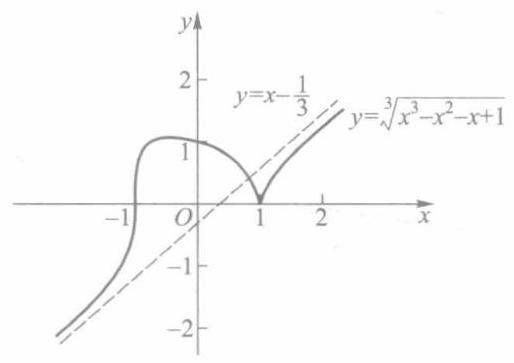
\includegraphics[width=.3\textwidth]{images/P047.jpg}
	\caption{图 $6-16$}
	\label{fig:P047}
\end{figure}

\end{solution}

\subsection{习题 6.6}

按函数作图步骤,作下列函数图像:

(1) \(y = {x}^{3} + 6{x}^{2} - {15x} - {20}\) ;

(2) \(y = \frac{{x}^{3}}{2{\left( 1 + x\right) }^{2}}\) ;

(3) \(y = x - 2\arctan x\) ;

(4) \(y = x{\mathrm{e}}^{-x}\) ;

(5) \(y = 3{x}^{5} - 5{x}^{3}\) ;

(6) \(y = {\mathrm{e}}^{-{x}^{2}}\) ;

(7) \(y = \left( {x - 1}\right) {x}^{\frac{2}{3}}\) ;

(8) \(y = {\left| x\right| }^{\frac{2}{3}}{\left( x - 2\right) }^{2}\) .

\section{方程的近似解}

在实际应用中, 常常求方程
\[
f\left( x\right)  = 0 \tag{1}
\]
的解.而方程求解的方法主要有两种:解析法和数值法.解析法也称为公式法, 得到的解是精确的, 比如一元二次方程的求解公式. 然而并不是所有的方程的根都能通过这种方法而求得. 法国著名数学家伽罗瓦 (Galois) 在 19 世纪就证明了形如
\[
y = {a}_{n}{x}^{n} + {a}_{n - 1}{x}^{n - 1} + \cdots  + {a}_{0} = 0\;\left( {{a}_{n} \neq  0}\right)
\]
的代数方程,当 \(n \geq  5\) 时,一般不存在求解公式. 因此对于一般方程,我们必须寻求其他的求解方法.

下面我们介绍一种数值解法一牛顿切线法.

设 \(f\) 为 \(\left\lbrack  {a,b}\right\rbrack\) 上的二阶可导函数,满足
\[
{f}^{\prime }\left( x\right)  \cdot  {f}^{\prime \prime }\left( x\right)  \neq  0,\;f\left( a\right)  \cdot  f\left( b\right)  < 0.
\]
牛顿切线法的基本思想是构造一收敛点列 \(\left\{  {x}_{n}\right\}\) ,使其极限 \(\mathop{\lim }\limits_{{n \rightarrow  \infty }}{x}_{n} = \xi\) 恰好是方程 (1) 的解. 因此当 \(n\) 充分大时, \({x}_{n}\) 可作为 \(\xi\) 的近似值. 下面分四种情形进行讨论.

(1)设 \({f}^{\prime }\left( x\right)  < 0,{f}^{\prime \prime }\left( x\right)  > 0\) . 从而有 \(f\left( a\right)  > 0,f\left( b\right)  < 0\) ,并设 \(f\left( \xi \right)  = 0\) . 令
\[
{x}_{0} = a,{x}_{n} = {x}_{n - 1} - \frac{f\left( {x}_{n - 1}\right) }{{f}^{\prime }\left( {x}_{n - 1}\right) },n = 1,2,\cdots . \tag{2}
\]
因为 \({f}^{\prime \prime }\left( x\right)  > 0\) ,所以 \(f\) 为 \(\left\lbrack  {a,b}\right\rbrack\) 上的严格凸函数,由定理 6.14
\[
f\left( x\right)  > f\left( a\right)  + {f}^{\prime }\left( a\right) \left( {x - a}\right) ,x \in  (a,b\rbrack . \tag{3}
\]
设 \({x}_{0} = a\) ,则 \(y = f\left( x\right)\) 在点 \(a\) 的切线与 \(x\) 轴的交点为
\[
{x}_{1} = a - \frac{f\left( a\right) }{{f}^{\prime }\left( a\right) } = {x}_{0} - \frac{f\left( {x}_{0}\right) }{{f}^{\prime }\left( {x}_{0}\right) }.
\]
由 (3) 式可知 \(f\left( {x}_{1}\right)  > 0\) (见图 6-17(1)).

以 \(\left\lbrack  {{x}_{1},b}\right\rbrack\) 代替 \(\left\lbrack  {a,b}\right\rbrack\) 重复上述步骤可得 \(y = f\left( x\right)\) 在点 \({x}_{1}\) 的切线与 \(x\) 轴交点为
\[
{x}_{2} = {x}_{1} - \frac{f\left( {x}_{1}\right) }{{f}^{\prime }\left( {x}_{1}\right) },
\]
其中 \(f\left( {x}_{2}\right)  > 0,a = {x}_{0} < {x}_{1} < {x}_{2} < \xi  < b\) .

如此继续上述过程可得如 (2) 式确定的点列 \(\left\{  {x}_{n}\right\}\) . 显然 \(\left\{  {x}_{n}\right\}\) 严格递增且有上界,故可设 \(\mathop{\lim }\limits_{{n \rightarrow  \infty }}{x}_{n} = c\) . 由于 \(f\) 和 \({f}^{\prime }\) 连续,对 (2) 式取极限,得
\[
c = c - \frac{f\left( c\right) }{{f}^{\prime }\left( c\right) }.
\]
因而有 \(f\left( c\right)  = 0\) . 由 \(f\) 严格单调,可知方程 (1) 的解唯一,从而 \(c = \xi\) .

最后我们估计以 \({x}_{n}\) 作为 \(\xi\) 的近似值的误差. 由中值定理
\[
f\left( {x}_{n}\right)  = f\left( {x}_{n}\right)  - f\left( \xi \right)  = {f}^{\prime }\left( \eta \right) \left( {{x}_{n} - \xi }\right) ,{x}_{n} < \eta  < \xi ,
\]
因而
\[
{x}_{n} - \xi  = \frac{f\left( {x}_{n}\right) }{{f}^{\prime }\left( \eta \right) }.
\]
\begin{figure}
	\centering
	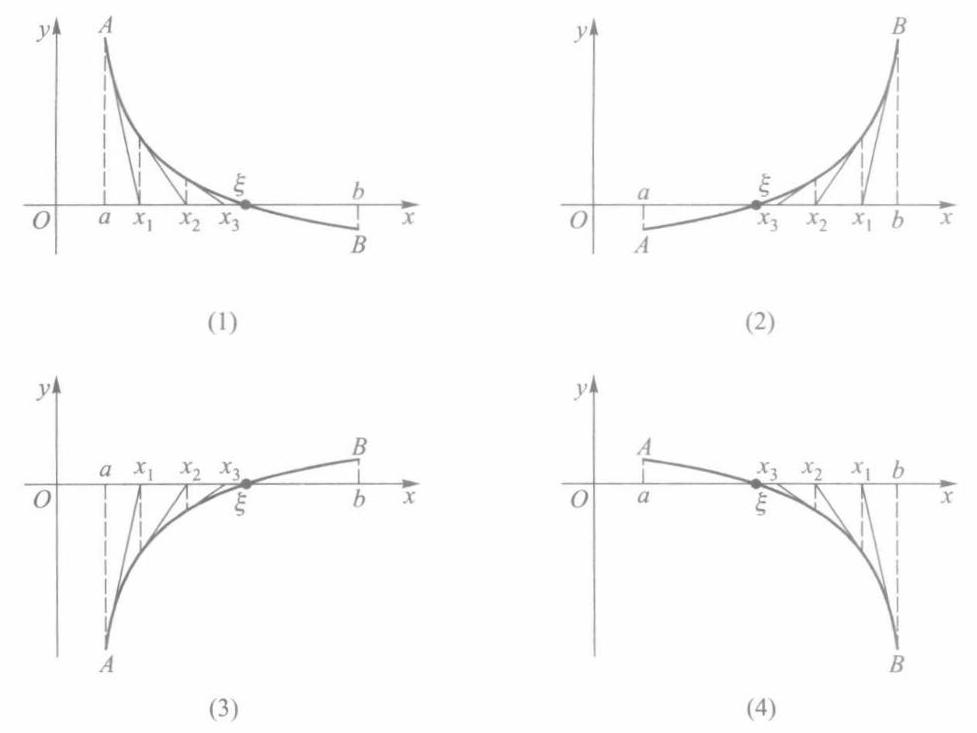
\includegraphics[width=.3\textwidth]{images/P048.jpg}
	\caption{图 $6-17$}
	\label{fig:P048}
\end{figure}

记 \(m = \mathop{\min }\limits_{{x \in  \left\lbrack  {a,b}\right\rbrack  }}\left\{  \left| {{f}^{\prime }\left( x\right) }\right| \right\}\) ,则
\[
\left| {{x}_{n} - \xi }\right|  \leq  \frac{\left| f\left( {x}_{n}\right) \right| }{m}. \tag{4}
\]
读者可类似讨论余下三种情形:

(2) \({f}^{\prime }\left( x\right)  > 0,{f}^{\prime \prime }\left( x\right)  > 0\) ,这时又有 \(f\left( a\right)  < 0,f\left( b\right)  > 0\) ;

(3) \({f}^{\prime }\left( x\right)  > 0,{f}^{\prime \prime }\left( x\right)  < 0\) ,这时又有 \(f\left( a\right)  < 0,f\left( b\right)  > 0\) ;

(4) \({f}^{\prime }\left( x\right)  < 0,{f}^{\prime \prime }\left( x\right)  < 0\) ,这时又有 \(f\left( a\right)  > 0,f\left( b\right)  < 0\) .

这三种情形的图像分别如图 6-17 中的(2)、(3)、(4)所示. 对它们同样能构造数列 (2), 并可证明其极限是方程 (1) 的解. 只是在 (2)、(4) 两种情形下, 应改取 \({x}_{0} = b\) ,相应得到的 \(\left\{  {x}_{n}\right\}\) 是单调递减的.

%例
\begin{example}
用牛顿切线法求方程 \({x}^{3} - 2{x}^{2} - {4x} - 7 = 0\) 的近似解,使误差不超过 0.01 .

\end{example}
%解
\begin{solution}
设 \(f\left( x\right)  = {x}^{3} - 2{x}^{2} - {4x} - 7\) . 求得导数
\[
{f}^{\prime }\left( x\right)  = 3{x}^{2} - {4x} - 4 = \left( {{3x} + 2}\right) \left( {x - 2}\right) ,
\]
\[
{f}^{\prime \prime }\left( x\right)  = {6x} - 4\text{ . }
\]
容易检验 \(x =  - \frac{2}{3}\) 为极大值点, \(x = 2\) 为极小值点,并且 \(f\left( {-\frac{2}{3}}\right)  < 0\) . 又因
\[
\mathop{\lim }\limits_{{x \rightarrow   - \infty }}f\left( x\right)  =  - \infty ,
\]
\(\mathop{\lim }\limits_{{x \rightarrow   + \infty }}f\left( x\right)  =  + \infty\) ,所以方程 \(f\left( x\right)  = 0\) 有且只有一个根.

注意到 \(f\left( 3\right)  =  - {10} < 0,f\left( 4\right)  = 9 > 0\) ,因而方程的根 \(\xi  \in  \left( {3,4}\right)\) . 由于在 \(\left\lbrack  {3,4}\right\rbrack\) 上 \({f}^{\prime }\left( x\right)\)  \(> 0\) , \({f}^{\prime \prime }\left( x\right)  > 0\) ,因此它属于情形 (2),如图 6-18 所示. 从点 \(B\left( {4,9}\right)\) 作切线与 \(x\) 轴相交于
\[
{x}_{1} = 4 - \frac{f\left( 4\right) }{{f}^{\prime }\left( 4\right) } = 4 - \frac{9}{28} \approx  {3.68}.
\]
\begin{figure}
    \centering
    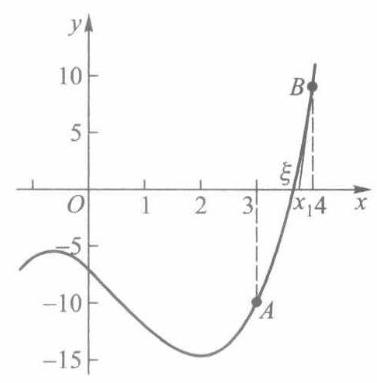
\includegraphics[width=.3\textwidth]{images/P049.jpg}
    \caption{图 $6-18$}
    \label{fig:P049}
\end{figure}

我们来估计以 \({x}_{1}\) 代替 \(\xi\) 的误差: \({f}^{\prime }\left( x\right)\) 在 \(\left\lbrack  {3,4}\right\rbrack\) 上的最小值为 \(m = {11}\) ,而 \(f\left( {x}_{1}\right)  \approx  f\left( {3.68}\right)  \approx  {1.03}\) ,由误差估计公式 (4)得
\[
\left| {{x}_{1} - \xi }\right|  \leq  \frac{\left| f\left( {x}_{1}\right) \right| }{m} \approx  \frac{1.03}{11},
\]
而 \(\frac{1.03}{11} > {0.01}\) ,因此尚不合要求.

再在点 \({B}^{\prime }\left( {{x}_{1},f\left( {x}_{1}\right) }\right)\) 作切线,求得
\[
{x}_{2} = {x}_{1} - \frac{f\left( {x}_{1}\right) }{{f}^{\prime }\left( {x}_{1}\right) } = {3.68} - \frac{1.03}{21.9} \approx  {3.63}.
\]
由于 \(f\left( {x}_{2}\right)  =  - {0.042}\) ,此时
\[
\left| {{x}_{2} - \xi }\right|  \leq  \frac{\left| f\left( {x}_{2}\right) \right| }{m} \approx  \frac{0.042}{11} < {0.01},
\]
因此取 \(\xi  \approx  {3.63}\) 已能达到所要求的精确度.
\end{solution}


\subsection{习题 6.7}

1. 求 \(\frac{{x}^{3}}{3} - {x}^{2} + 2 = 0\) 的实根,精确到三位有效数字.

2. 求方程 \(x = {0.538}\sin x + 1\) 的根的近似值,精确到 0.001 .

\section{第六章总练习题}

1. 证明: 若 \(f\left( x\right)\) 在有限开区间(a, b)上可导,且 \(\mathop{\lim }\limits_{{x \rightarrow  {a}^{ + }}}f\left( x\right)  = \mathop{\lim }\limits_{{x \rightarrow  {b}^{ - }}}f\left( x\right)\) ,则至少存在一点 \(\xi  \in  \left( {a,b}\right)\) , 使 \({f}^{\prime }\left( \xi \right)  = 0\) .

2. 证明: 若 \(x > 0\) ,则

(1) \(\sqrt{x + 1} - \sqrt{x} = \frac{1}{2\sqrt{x + \theta \left( x\right) }}\) ,其中 \(\frac{1}{4} \leq  \theta \left( x\right)  \leq  \frac{1}{2}\) ；

(2) \(\mathop{\lim }\limits_{{x \rightarrow  {0}^{ + }}}\theta \left( x\right)  = \frac{1}{4},\mathop{\lim }\limits_{{x \rightarrow   + \infty }}\theta \left( x\right)  = \frac{1}{2}\) .

3. 设函数 \(f\) 在 \(\left\lbrack  {a,b}\right\rbrack\) 上连续,在(a, b)上可导,且 \(a \cdot  b > 0\) . 证明存在 \(\xi  \in  \left( {a,b}\right)\) ,使得
\[
\frac{1}{a - b}\left| \begin{matrix} a & b \\  f\left( a\right) & f\left( b\right)  \end{matrix}\right|  = f\left( \xi \right)  - \xi {f}^{\prime }\left( \xi \right) .
\]

4. 设 \(f\) 在 \(\left\lbrack  {a,b}\right\rbrack\) 上三阶可导,证明存在 \(\xi  \in  \left( {a,b}\right)\) ,使得
\[
f\left( b\right)  = f\left( a\right)  + \frac{1}{2}\left( {b - a}\right) \left\lbrack  {{f}^{\prime }\left( a\right)  + {f}^{\prime }\left( b\right) }\right\rbrack   - \frac{1}{12}{\left( b - a\right) }^{3}{f}^{\prime \prime \prime }\left( \xi \right) .
\]

5. 对 \(f\left( x\right)  = \ln \left( {1 + x}\right)\) 应用拉格朗日中值定理,试证: 对 \(x > 0\) ,有
\[
0 < \frac{1}{\ln \left( {1 + x}\right) } - \frac{1}{x} < 1.
\]

6. 设 \({a}_{1},{a}_{2},\cdots ,{a}_{n}\) 为 \(n\) 个正数,且
\[
f\left( x\right)  = {\left( \frac{{a}_{1}^{x} + {a}_{2}^{x} + \cdots  + {a}_{n}^{x}}{n}\right) }^{\frac{1}{x}}.
\]
证明: (1) \(\mathop{\lim }\limits_{{x \rightarrow  0}}f\left( x\right)  = \sqrt[n]{{a}_{1}{a}_{2}\cdots {a}_{n}}\) ;

(2) \(\mathop{\lim }\limits_{{x \rightarrow   + \infty }}f\left( x\right)  = \max \left\{  {{a}_{1},{a}_{2},\cdots ,{a}_{n}}\right\}\) .

7. 求下列极限:

(1) \(\mathop{\lim }\limits_{{x \rightarrow  {1}^{ - }}}{\left( 1 - {x}^{2}\right) }^{1/\ln \left( {1 - x}\right) }\) ;

(2) \(\mathop{\lim }\limits_{{x \rightarrow  0}}\frac{x{\mathrm{e}}^{x} - \ln \left( {1 + x}\right) }{{x}^{2}}\) ;

(3) \(\mathop{\lim }\limits_{{x \rightarrow  0}}\frac{{x}^{2}\sin \frac{1}{x}}{\sin x}\) .

8. 设 \(h > 0\) ,函数 \(f\) 在 \(U\left( {a;h}\right)\) 上具有 \(n + 2\) 阶连续导数,且 \({f}^{\left( n + 2\right) }\left( a\right)  \neq  0,f\) 在 \(U\left( {a;h}\right)\) 上的泰勒公式为
\[
f\left( {a + h}\right)  = f\left( a\right)  + {f}^{\prime }\left( a\right) h + \cdots  + \frac{{f}^{\left( n\right) }\left( a\right) }{n!}{h}^{n} + \frac{{f}^{\left( n + 1\right) }\left( {a + {\theta h}}\right) }{\left( {n + 1}\right) !}{h}^{n + 1},0 < \theta  < 1.
\]
证明: \(\mathop{\lim }\limits_{{h \rightarrow  0}}\theta  = \frac{1}{n + 2}\) .

9. 设 \(k > 0\) ,试问 \(k\) 为何值时,方程 \(\arctan x - {kx} = 0\) 有正实根.

10. 证明: 对任一多项式 \(p\left( x\right)\) ,一定存在 \({x}_{1}\) 与 \({x}_{2}\) ,使 \(p\left( x\right)\) 在 \(\left( {-\infty ,{x}_{1}}\right)\) 与 \(\left( {{x}_{2}, + \infty }\right)\) 上分别严格单调.

11. 讨论函数
\[
f\left( x\right)  = \left\{  \begin{array}{ll} \frac{x}{2} + {x}^{2}\sin \frac{1}{x}, & x \neq  0, \\  0, & x = 0, \end{array}\right.
\]

(1)在 \(x = 0\) 点是否可导?

(2)是否存在 \(x = 0\) 的一个邻域,使 \(f\) 在该邻域上单调？

12. 设函数 \(f\) 在 \(\left\lbrack  {a,b}\right\rbrack\) 上二阶可导, \({f}^{\prime }\left( a\right)  = {f}^{\prime }\left( b\right)  = 0\) . 证明存在一点 \(\xi  \in  \left( {a,b}\right)\) ,使得
\[
\left| {{f}^{\prime \prime }\left( \xi \right) }\right|  \geq  \frac{4}{{\left( b - a\right) }^{2}}\left| {f\left( b\right)  - f\left( a\right) }\right| .
\]

13. 设函数 \(f\) 在 \(\left\lbrack  {0,a}\right\rbrack\) 上具有二阶导数,且 \(\left| {{f}^{\prime \prime }\left( x\right) }\right|  \leq  M,f\) 在(0, a)上取得最大值. 试证
\[
\left| {{f}^{\prime }\left( 0\right) }\right|  + \left| {{f}^{\prime }\left( a\right) }\right|  \leq  {Ma}.
\]

14. 设 \(f\) 在 \(\lbrack 0, + \infty )\) 上可微,且 \(0 \leq  {f}^{\prime }\left( x\right)  \leq  f\left( x\right) ,f\left( 0\right)  = 0\) . 证明: 在 \(\lbrack 0, + \infty )\) 上 \(f\left( x\right)  \equiv  0\) .

15. 设 \(f\left( x\right)\) 满足 \({f}^{\prime \prime }\left( x\right)  + {f}^{\prime }\left( x\right) g\left( x\right)  - f\left( x\right)  = 0\) ,其中 \(g\left( x\right)\) 为任一函数.

证明: 若 \(f\left( {x}_{0}\right)  = f\left( {x}_{1}\right)  = 0\)  \(\left( {{x}_{0} < {x}_{1}}\right)\) ,则 \(f\) 在 \(\left\lbrack  {{x}_{0},{x}_{1}}\right\rbrack\) 上恒等于 0 .

16. 证明: 定圆内接正 \(n\) 边形面积将随 \(n\) 的增加而增加.

17. 证明: \(f\) 为 \(I\) 上凸函数的充要条件是对任何 \({x}_{1},{x}_{2} \in  I\) ,函数
\[
\varphi \left( \lambda \right)  = f\left( {\lambda {x}_{1} + \left( {1 - \lambda }\right) {x}_{2}}\right)
\]
为 \(\left\lbrack  {0,1}\right\rbrack\) 上的凸函数

18. 证明:

(1) 设 \(f\) 在 \(\left( {a, + \infty }\right)\) 上可导,若 \(\mathop{\lim }\limits_{{x \rightarrow   + \infty }}f\left( x\right) ,\mathop{\lim }\limits_{{x \rightarrow   + \infty }}{f}^{\prime }\left( x\right)\) 都存在,则
\[
\mathop{\lim }\limits_{{x \rightarrow   + \infty }}{f}^{\prime }\left( x\right)  = 0.
\]

(2) 设 \(f\) 在 \(\left( {a, + \infty }\right)\) 上 \(n\) 阶可导. 若 \(\mathop{\lim }\limits_{{x \rightarrow   + \infty }}f\left( x\right)\) 和 \(\mathop{\lim }\limits_{{x \rightarrow   + \infty }}{f}^{\left( n\right) }\left( x\right)\) 都存在,则
\[
\mathop{\lim }\limits_{{x \rightarrow   + \infty }}{f}^{\left( k\right) }\left( x\right)  = 0\left( {k = 1,2,\cdots ,n}\right) .
\]

19. 设 \(f\) 为 \(\left( {-\infty , + \infty }\right)\) 上的二阶可导函数. 若 \(f\) 在 \(\left( {-\infty , + \infty }\right)\) 上有界,则存在 \(\xi  \in  \left( {-\infty , + \infty }\right)\) , 使 \({f}^{\prime \prime }\left( \xi \right)  = 0\) .

\section{第六章综合自测题}

